%%%%%%%%%%%%%%%%%%%%%%%%%%%%%%%%%%%%%%%%%%%%%%%%%%%%%%%%%%%%%%%%%%%%%%%%%%
% 
% Sverdrup is not a hero. He exists to point to the Cross. He doesn't stand on a pedestal. 
%
% At the same time, it's fun to watch him point. 
% 
% What Sverdrup feared was not the death of the congregation, but its successful replacement by machinery.
%
%%%%%%%%%%%%%%%%%%%%%%%%%%%%%%%%%%%%%%%%%%%%%%%%%%%%%%%%%%%%%%%%%%%%%%%%%%
%
% Who wrote the sermons?
%
% Do not attempt sermon-by-sermon authorship assignments in this book.
%
% Respect the original text! 
%
%
% Translator's triangle:
% * Structural fidelity – preserving the order, logical movement, and rhetorical shape of the 1871 Danish text as far as English permits.
% * Emotional equivalence – preserving the moral and rhetorical force of the original, even where English must take a different form to convey it.
% * Theological precision – rendering key doctrinal terms consistently and without interpretive softening.
%
% No attempt has been made to modernize the theology, harmonize the text with familiar English Bible versions, or embellish the style of the source.
%
%%%%%%%%%%%%%%%%%%%%%%%%%%%%%%%%%%%%%%%%%%%%%%%%%%%%%%%%%%%%%%%%%%%%%%%%%%

% FIXME: Start  over and look for caps  capitalization. 

% FIXME: Start over and correct for "reduced emotional volatility." This hazard was discovered 143 pages into the text.

% For refined edits:
% * the offending English clause
% * no recommendation without showing the Danish pressure it answers to
% * the justification
% * a primary and alternative fix


% master.tex
\documentclass[12pt]{article}

% -------------------- Page + typography --------------------
\usepackage[letterpaper,margin=1in]{geometry}
\usepackage[T1]{fontenc}
\usepackage[utf8]{inputenc} % safe for pdfLaTeX
\usepackage{lmodern}
\usepackage{microtype}
\usepackage{setspace}
\usepackage{graphicx}
\usepackage{parskip}        % no paragraph indent; spacing between paragraphs

\usepackage{tabularx}
\usepackage{ragged2e}

\usepackage{xcolor}


\usepackage{comment}

\usepackage{pdfpages}

% -------------------- Links (optional) --------------------
\usepackage[hidelinks]{hyperref}

% -------------------- TOC depth --------------------
\setcounter{tocdepth}{3}


% ---------- Header/footer ----------
\usepackage{fancyhdr}
\pagestyle{fancy}
\fancyhf{}
\renewcommand{\headrulewidth}{0.2pt}
%\fancyhead[L]{\small Sverdrup — Working Translation}
%\fancyhead[R]{\small \leftmark}
\fancyfoot[C]{\small \thepage}

\fancypagestyle{plain}{%
  \fancyhf{}
  \renewcommand{\headrulewidth}{0.2pt}
  \fancyhead[L]{\small Sverdrup — Working Translation}
  \fancyhead[R]{\small \nouppercase{\rightmark}}
  \fancyfoot[C]{\small \thepage}
}

\newenvironment{psalm}{
  \parindent=0pt
  \leftskip=1.5em
  \rightskip=1.5em
  \parskip=0.6\baselineskip
}{\par}


\definecolor{oxblood}{RGB}{74, 0, 0}
\begin{document}

% ==========================================================
% Title Page (English, modeled on the scanned 1910 title page)
% ==========================================================
\begin{titlepage}
    \centering
    \vspace*{1.5in}

    {\Large Professors Oftedal and Sverdrup\par}
    \vspace{0.25in}

    {\large Teachers of Theology at Augsburg Seminary\par}
    \vspace{0.25in}

    {\LARGE\bfseries Spirit and Life\par}
    \vspace{0.10in}
    {\large (Aand og Liv)\par}

    \vspace{0.25in}

    {\large Sermons on the Gospels of All Three Lectionary Cycles\par}
    \vspace{0.15in}
    {\large (Prædikener over Alle tre Tekstrækkers Evangelier)\par}

    \vfill

    {\small Minneapolis, Minnesota\par}
    {\small Published by The Free Church Book Concern\par}
    {\small 1898\par}

    \vspace{0.5in}

\end{titlepage}


% ======================
% Front matter: TOC
% ======================


\cleardoublepage
\thispagestyle{empty}


\begin{center}
  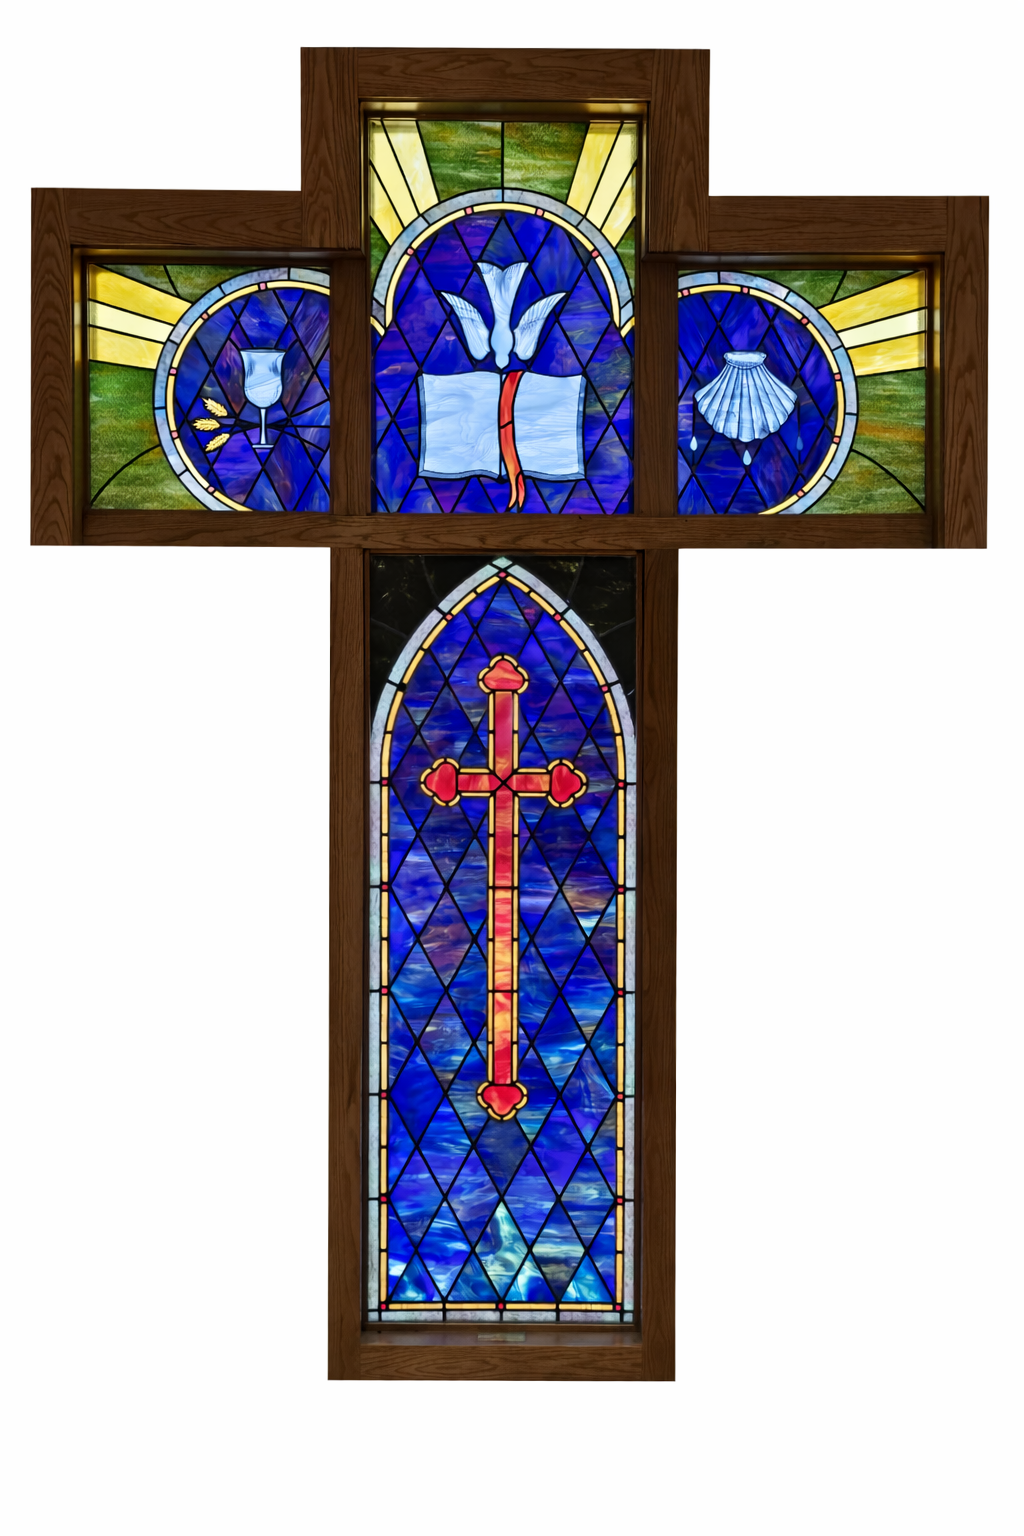
\includegraphics[height=0.85\textheight,keepaspectratio]{cross.png}
\end{center}

\vfill
{\small\itshape “I see my bond of debt nailed fast high on the cross.”}

Southwest window\\
Our Saviour's Lutheran Church \\
Thief River Falls, Minnesota\\ 

\cleardoublepage


\pagenumbering{roman}


\cleardoublepage



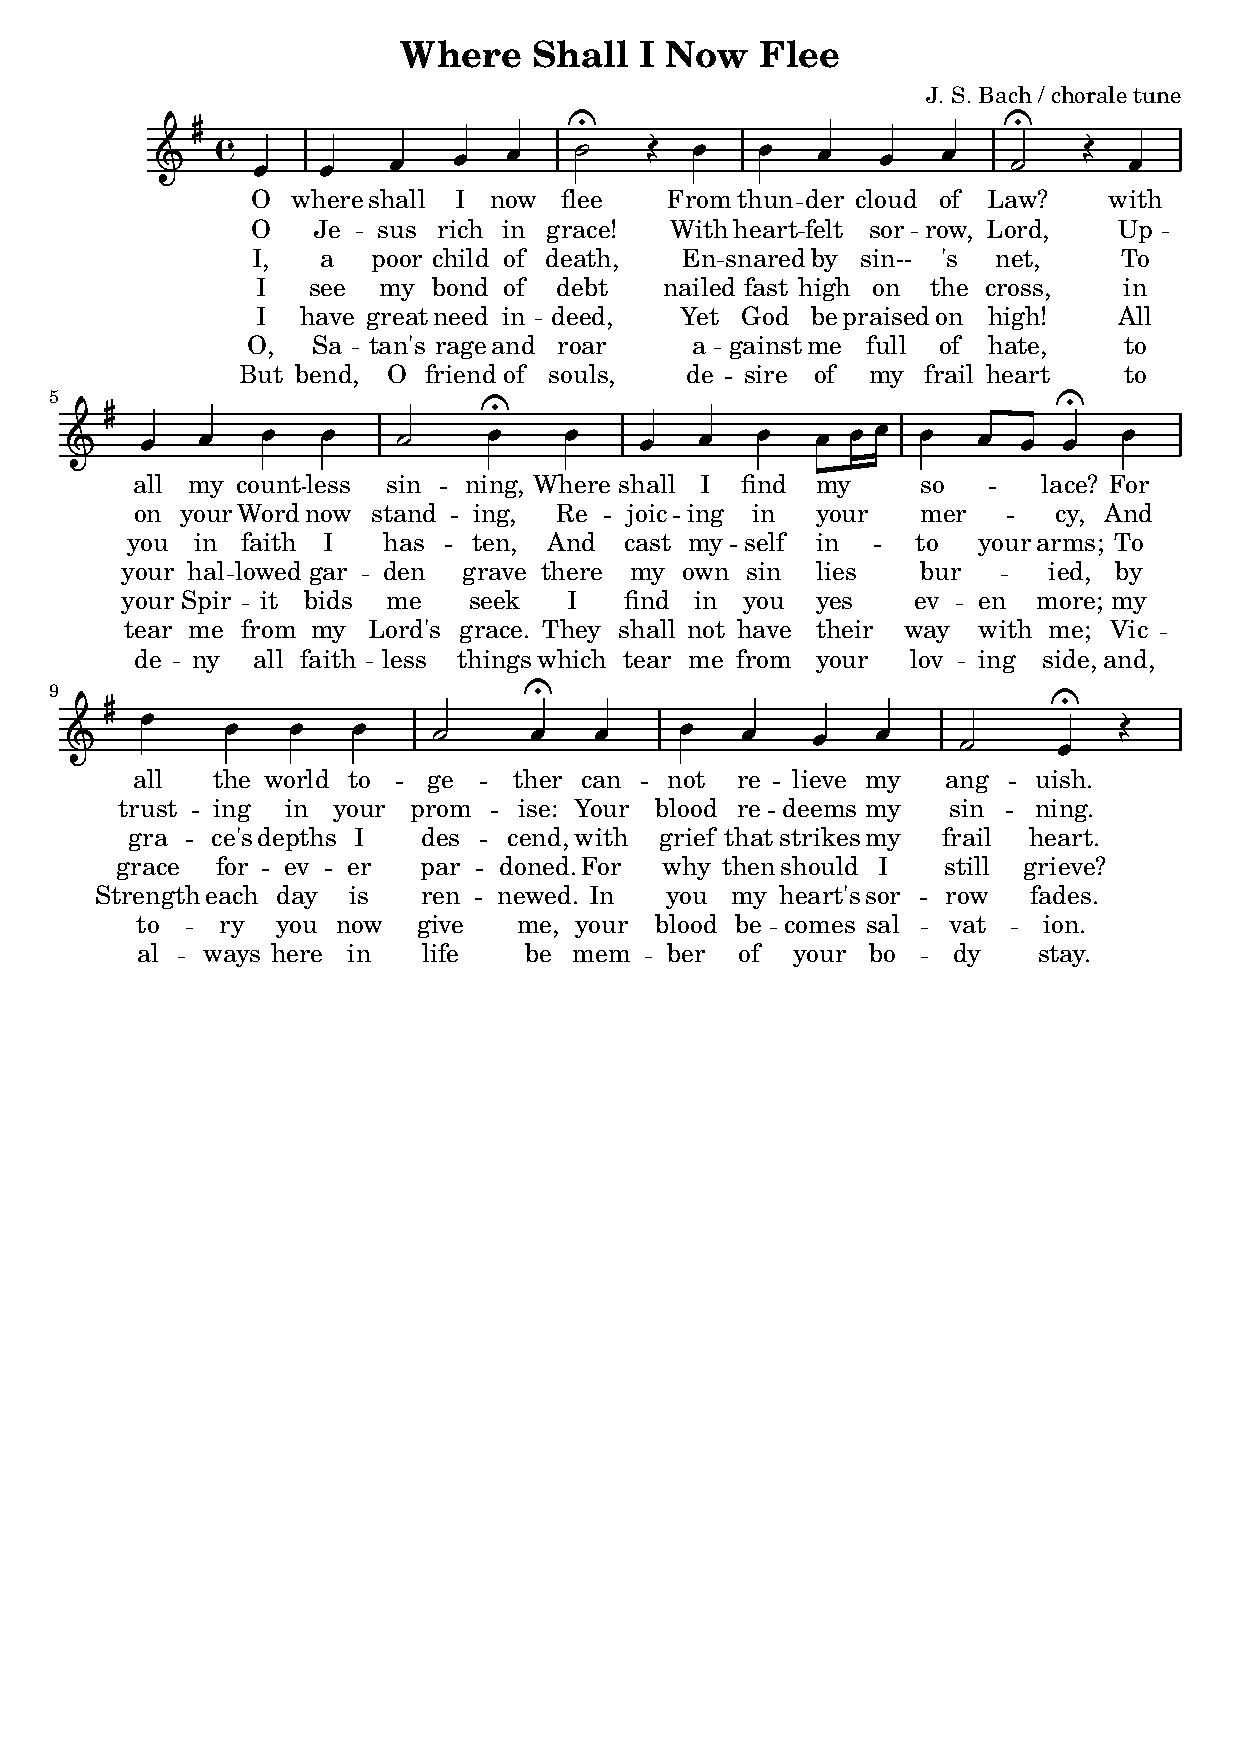
\includepdf[pages=1]{Hymn/Where_Shall_I_Now_Flee.pdf}

\begin{comment}
% Note that the English has been voiced against Auf meinen lieben Gott

\noindent
\begin{minipage}[t]{0.48\textwidth}
\RaggedRight
\begin{center}
Hvorhen skal jeg dog fly\\
Fra Lovens Tordensky\\
Med mine Synder mange,\\
Hvor skal jeg Trøsten fange?\\
Thi hele Verden vide\\
Ei lette kan min Kvide.\\[0.6em]

O Jesus, naaderig!\\
Med Hjertens Sorg til dig\\
Jeg paa dit Ord fremtræder,\\
Mig ved din Naade glæder,\\
Og tror, hvad du forjætter,\\
Dit Blod min Synd udsletter.\\[0.6em]

Jeg arme Dødsens Barn,\\
Omsnært af Syndens Garn,\\
Til dig i Troen haster,\\
Og i din Favn mig kaster,\\
I Naadens Dyb jeg sænker\\
Den Kval, som Hjertet krænker.\\[0.6em]

Jeg ser, mit Skylde-Brev\\
Til Korset naglet blev,\\
Og i din Grav i Haven,\\
Der er min Synd begraven\\
Til evig Skjul og Gjemme,\\
Hvi vil jeg mig da gremme?\\[0.6em]

Jeg meget har behov,\\
Men Gud ske evig Lov!\\
Alt, hvad jeg kan begjære,\\
Hos dig jeg faar, ja mere;\\
Min Kraft i dig jeg finder,\\
Hos dig min Sorg forsvinder.\\[0.6em]

Om Satans hele Magt\\
Sig hade mod mig lagt,\\
For mig fra dig at skille,\\
De faa ei, hvad de ville,\\
Thi du mig Seier giver,\\
Dit Blod min Frelse bliver.\\[0.6em]

Men bøi, o Sjæleven,\\
Min Hjertens Hu derhen,\\
At jeg maa alt modstride,\\
Som mig fra dig vil slide,\\
Og altid her i Live\\
Dit Legems Lem forblive.
\end{center}
\end{minipage}
\hfill
\begin{minipage}[t]{0.48\textwidth}
\RaggedRight
\begin{center}
Oh where shall I now flee\\
From thundercloud of Law\\
with all my countless sinning,\\
Where shall I find my solace?\\
For all the world together\\
Cannot relieve my anguish.\\[0.6em]

O Jesus, rich in grace!\\
With heartfelt sorrow, Lord;\\
Upon your Word now standing,\\
Rejoicing in your mercy,\\
And trusting in your promise:\\
Your blood redeems my sinning.\\[0.6em]

I, a poor child of death,\\
Ensnared by sin’s net,\\
To you in faith I hasten\\
And cast myself into your arms;\\
to grace’s depths I descend\\
The torment that wounds the heart.\\[0.6em]

I see my record of debt\\
Nailed fast to the cross,\\
And in your grave in the garden\\
There my sin lies buried,\\
Hidden away forever---\\
Then why should I still grieve?\\[0.6em]




I have great need indeed,\\
Yet God be praised on high!\\
All that I could desire\\
I find in you and more;\\
In you I find my strength,\\
In you my sorrow fades.\\[0.6em]

% Continue here...

Though Satan rage and roar \\
Against me full of hate,\\
To tear me away from you,\\
They shall not have their will;\\
For you give victory,\\
Your blood my salvation.\\[0.6em]

Now bend, O Prince of souls,\\
My heart’s desire toward this:\\
That I may resist all\\
Which would tear me from you,\\
And always here in life\\
Member of your body sealed .\\

\end{center}
\end{minipage}

\end{comment}

\cleardoublepage



\tableofcontents
\newpage


\input{TranslatorNote.tex}
\pagebreak
%\input{Forward/Forward.tex}
%\pagebreak

% ======================
% Main matter
% ======================
\pagenumbering{arabic}

\pagestyle{plain}
% First included file:
\input{Sermon1/Sermon1.tex}\pagebreak
\input{Sermon4/Sermon4.tex}\pagebreak
\input{Sermon8/Sermon8.tex}\pagebreak
\input{Sermon11/Sermon11.tex}\pagebreak
\input{Sermon14/Sermon14.tex}\pagebreak
\input{Sermon18/Sermon18.tex}\pagebreak
\input{Sermon22/Sermon22.tex}\pagebreak
\input{Sermon25/Sermon25.tex}\pagebreak
\input{Sermon29/Sermon29.tex}\pagebreak
\input{Sermon34/Sermon34.tex}\pagebreak
\input{Sermon39/Sermon39.tex}\pagebreak
\input{Sermon43/Sermon43.tex}\pagebreak
\input{Sermon47/Sermon47.tex}\pagebreak
\input{Sermon50/Sermon50.tex}\pagebreak
\input{Sermon55/Sermon55.tex}\pagebreak
\input{Sermon59/Sermon59.tex}\pagebreak
\input{Sermon64/Sermon64.tex}\pagebreak
\input{Sermon68/Sermon68.tex}\pagebreak
\input{Sermon71/Sermon71.tex}\pagebreak
\input{Sermon74/Sermon74.tex}\pagebreak
\input{Sermon77/Sermon77.tex}\pagebreak
\input{Sermon82/Sermon82.tex}\pagebreak
\input{Sermon85/Sermon85.tex}\pagebreak
\input{Sermon88/Sermon88.tex}\pagebreak
\input{Sermon92/Sermon92.tex}\pagebreak
\input{Sermon96/Sermon96.tex}\pagebreak
\input{Sermon101/Sermon101.tex}\pagebreak
\input{Sermon107/Sermon107.tex}\pagebreak
\input{Sermon111/Sermon111.tex}\pagebreak
\input{Sermon116/Sermon116.tex}\pagebreak
\input{Sermon120/Sermon120.tex}\pagebreak
\input{Sermon123/Sermon123.tex}\pagebreak
\input{Sermon127/Sermon127.tex}\pagebreak
\input{Sermon131/Sermon131.tex}\pagebreak
\input{Sermon135/Sermon135.tex}\pagebreak
\input{Sermon139/Sermon139.tex}\pagebreak
\input{Sermon143/Sermon143.tex}\pagebreak
\input{Sermon146/Sermon146.tex}\pagebreak
\input{Sermon149/Sermon149.tex}\pagebreak
\input{Sermon154/Sermon154.tex}\pagebreak
\input{Sermon158/Sermon158.tex}\pagebreak
\input{Sermon162/Sermon162.tex}\pagebreak
\input{Sermon166/Sermon166.tex}\pagebreak
\input{Sermon170/Sermon170.tex}\pagebreak


\section{Sixth Sunday after Trinity: The Mind of the Flesh Is Enmity Against God}

\begin{quote}

Matthew 5:27–37. You have heard that it was said to those of old: You shall not commit adultery. But I say to you that everyone who looks at a woman in order to desire her has already committed adultery with her in his heart. But if your right eye causes you to stumble, tear it out and cast it from you. For it is better for you that one of your members perish than that your whole body be cast into hell. And if your right hand causes you to stumble, cut it off and cast it from you. For it is better for you that one of your members perish than that your whole body be cast into hell. 

It has also been said that whoever divorces his wife shall give her a certificate of divorce. But I say to you that whoever divorces his wife, except on account of fornication, causes her to commit adultery, and whoever marries a divorced woman commits adultery. Again you have heard that it was said to those of old: You shall not swear falsely, but shall perform to the Lord your oaths. But I say to you, do not swear at all: neither by heaven, for it is God’s throne; nor by the earth, for it is his footstool; nor by Jerusalem, for it is the city of the great King. Neither shall you swear by your head, for you cannot make one hair white or black. But let your speech be yes, yes; no, no. Whatever is more than this comes from evil.

\end{quote}

\bigskip


To admit that human nature is corrupted from birth, “conceived in sin and born in iniquity,” incapable of all good and inclined to all evil, will always be hard and distasteful to flesh and blood. For alongside the evil we think we see so much that is great and noble in the human spirit and in human life that the word, “that which is born of the flesh is flesh,” becomes to us altogether incomprehensible and unreasonable.

Must there really be no one among us who is good? Should it not be possible for someone, with the help of the good that is in him, if only he will in earnest, to combat and overcome the evil and thus become acceptable before God? Is not human nature in its essence good, because it is created by God, and has he not precisely given us his Law in order to show us how we may oppose and cast off all the uncleanness and sin that on account of our corruptibility presses in upon us?

These and similar questions have at all times been raised by all whenever the holy demands of God’s Law, with their sharp edge, have begun to stir the conscience. Then the excuses begin. To let the Law do its work, to acknowledge sin, and to come to God begging for grace—this the carnal ego resists and will rather resort to every invention and every illusion than to “give oneself up in order to gain oneself,” to “surrender one’s life in order to gain a life.”

And when then God’s Law stands just as holy, just as unyielding in its demands, and man neither dares reject it nor will bow beneath its judgment, then the question becomes how by every kind of trimming and reinterpretation one may break off its sharp edge and thus establish, as it were, a truce between the conscience and the Law, a righteousness of one’s own between God and man.

This is what we all, according to the carnality and dishonesty of our nature, are daily more or less consciously tempted to do, and it was precisely this in which the scribes of the Jews, after many hundreds of years of study of the Law, had become masters.

By all manner of interpretations, reductions, regulations, and traditions they had brought matters so far that they could live on excellent terms with the Law and, in their own opinion, fulfill all its demands and thereby gain a right to blessedness.

But the high thoughts of man must be brought low and his self‑deception uncovered if salvation is to come. Therefore the Savior strikes again and again with heavy blows of the two‑edged sword of the Law against the self‑righteousness of the Jews and rebukes their carnal and corrupt art of interpretation.

“How neatly you set aside God’s commandment in order to keep your own ordinance,” he says in one place (Mark 7:9), and here in our text he uncovers this hypocrisy of theirs in relation to the two things that most of all reveal the sinful and corrupted nature of man: lust and dishonesty.

At all times, and not least in our own day, men have labored hard to present lust or fornication as something purely natural, purely human, something that is by no means sinful in itself, even if for reasons of expediency it ought to be limited or regulated. This is a thoroughly heathen thought, and it is therefore no wonder that fornication in all its most abominable forms everywhere is the distinguishing mark and curse of heathenism.

But the Pharisees also, who boasted in the Law and acknowledged it as a command from God, “You shall not commit adultery,” sought to bring about a compromise between their lust and God’s holy will, partly by considering only the letter of the Law and partly by adapting its demands to the requirements of human and civil conditions, as it is also so beautifully said in our own day.

The Lord shows them that not only the outward act of adultery is sin, but even the “looking at a woman in order to desire her.” That is to say: our innermost thoughts, our most natural desires—lust itself as part of our being—is sin. “That which is born of the flesh is flesh.” 

How then can anyone stand? 

If the innermost thoughts and desires of my corrupt nature stand opposed to the very nature of the incorruptible God so that he must cast me away from himself in the judgment—where then is salvation? 

\textbf{At Golgotha there is salvation. God’s Word wounds, but it also heals.}

“For what the Law could not do, in that it was weak through the flesh, God did: sending his own Son in the likeness of sinful flesh and for sin, he condemned sin in the flesh, that the requirement of the Law might be fulfilled in us who walk not according to the flesh but according to the Spirit.”

God’s Word kills, but it also makes alive. And that which is born of the Spirit is spirit. He who in his distress has fled to Christ and through faith in him has received a new life, a new nature, does not steal away from the Law like the Pharisees and nominal Christians, but daily and in all earnestness allows the Law to condemn sin in his flesh, in order daily anew to flee to Golgotha and be washed clean in the blood of the Son of God.

Thus the Law on the one hand exposes sin, and on the other shows the believer what fruits faith must bear. This is what Jesus meant to teach the self-righteous Jews when he set forth the Law—and what his Holy Spirit teaches us daily.

But in this matter there is no compromise, no reconciliation with the world or with the so‑called purely human. It is precisely this purely human, this natural element, which in Scripture is called flesh, and of which it is said that the mind of the flesh is enmity against God.

Therefore Jesus rebukes the scribes for their careless and immoral view of the relation of marriage, namely that a man may divorce his wife if only he gives her a certificate of divorce. Assuredly the Pharisees maintained that it was necessary to adapt oneself thus far to the demands of imperfect human conditions and as it were regulate them and prevent greater excesses.

But that in its foundation this was only to reduce God’s demand in order to accommodate the lust of human nature and thus give ungodliness the appearance of righteousness—this the Lord clearly shows when he expressly declares that through such frivolous divorces there simply arises an adulterous relation.

This was surely hard for the Pharisees to hear and shameful, as when he asked that the one among them who was without sin should cast the first stone. It is therefore no wonder that in their bitterness they killed him; but his word was nevertheless truth.

One man and one woman. “The man shall leave his father and mother and cling to his wife, and the two shall be one flesh.” So it was from the beginning, and so it is God’s truth to this day, however much also the Pharisees and Sadducees of our own time seek to conceal it and by compromising with Satan and the world and the fornication of human nature dissolve the Word of God and even pronounce the church’s blessing over unions which the Lord himself calls adultery.

To divorce one’s wife is—like all other fornication—natural and human enough, but it is sinful and irreconcilable.

With the same uncompromising clarity the Savior speaks of the other evil mark of human nature: dishonesty. The lie is a part of our nature after him who is the father of lies. We lie to one another and to ourselves. Therefore men feel the need to swear, because they do not trust one another.

Should this be necessary among those who are born of God, who always remember his most holy presence? Should not their yes and their no be a holier assurance than the most solemn oaths of worldly men?

Therefore the Lord says: “You shall not swear at all”—a word which also in our time, when so many wish to mingle Christianity with authority and civilization, needs seriously to be laid to heart.

Cleanse yourselves. Flee from sin in every form. 

Flee from fornication. 

Become pure. 

Put away lying and speak truth with your neighbor, since we are members one of another. Add nothing to and take nothing from God’s holy Law lest he punish you. Do not be yoked together with unbelievers. For what fellowship has righteousness with unrighteousness? What communion has light with darkness?

Is not the mind of the flesh enmity against God?

\pagebreak

\section{Seventh Sunday after Trinity: The True Banquet}


\begin{quote}

Luke 14:12–15. And he said also to the one who had invited him: When you make a dinner or a supper, do not invite your friends, your brothers, your relatives, or rich neighbors, lest they also invite you again and you receive repayment. But when you make a feast, invite the poor, the crippled, the lame, the blind. Then you shall be blessed; for they have nothing with which to repay you, but it shall be repaid to you at the resurrection of the righteous. But when one of those who sat with him at table heard this, he said to him: Blessed is the one who eats bread in the kingdom of God.

\end{quote}

\bigskip


According to this account and the one that precedes it, Jesus is a remarkable guest. He was in the house of a Pharisee and was sitting at the table with him. There he took the occasion to speak grave words both to the guests and to the host. To the guests he spoke about taking the lowest place and humbling themselves. To the host he spoke about whom he ought to invite when he gives a feast.

There is a sharp edge and sober seriousness in both of these table speeches. The guests were likely among those who sought honor from people rather than the honor that comes from the one God. And the host, who was a Pharisee, probably cared more for the reward he could receive at once than for the reward that lies hidden with the heavenly Father and will be revealed only on the day of Jesus Christ in the resurrection of the righteous.

The host invited friends and brothers and relatives and wealthy neighbors who could give a feast in return; but he did not think of making for himself such friends by means of unrighteous mammon as might receive him into the eternal dwellings.

Therefore the intention of Jesus Christ is not merely to give rules about what kinds of social gatherings may or may not be suitable within the congregation of God. His intention is to rebuke that whole form of religion and morality, that entire outlook on life and manner of living, which strives after earthly, temporal, and perishable advantages and distinctions while forgetting the eternal responsibility and the eternal and imperishable glory.

Large gatherings or small gatherings that pass, as it were, from one household to another in turn, and in which a brief earthly enjoyment is all that is sought and given, are not what Jesus has in mind. He always has eternity in view. And when he sees how people squander precious hours of grace through fleeting pleasures and empty diversions, and how they move thoughtlessly toward death and eternity, he has compassion on such misery. For he sees that they move along the edge of the abyss, only a hair’s breadth from eternal judgment.

He sees a spirit that cannot endure. Therefore he warns against gatherings that have no worth for eternity, and he commends a wholly different kind of gathering—one ordered entirely in view of the demands of eternal responsibility.

To feed the rich while the hungry and poor are sent away empty‑handed—that is the spirit of the world and the wisdom of the world. It receives its reward in this world and its comfort in the present time. But it is a grave folly for the person whose eye is directed toward what is eternal. For in the judgment it counts for nothing that a person has enjoyed life with his friends if he has neglected to clothe the naked, feed the hungry, and visit the sick and the sorrowful.

Give feasts for the poor. Help those who cannot help themselves. This is the counsel of Jesus to those who wish to give the right kind of feast. To take earthly wealth and turn it into eternal treasure, into a heavenly treasure that moth and rust cannot destroy and that no thief’s hand can carry away—this is the wisdom of the heavenly household and the true spiritual economy.

And this happens in a very simple and trusting way: the poor person’s hand becomes your bank, and you dare to entrust your means there. Whoever does this for God’s sake has stored both principal and interest with the Lord, and it will be returned to him in the resurrection of the righteous.

How can this be, and how does it hold together? If it could be explained to human reason, and if it were taken in a merely earthly way, it would become nothing more than a new kind of Phariseeism that imagines salvation can be purchased by almsgiving. That is not what Jesus intends.

It is not a bargain. It is not clever calculation. It is something entirely different: the boldness of faith and the self‑giving of love. For even if someone were to give all his possessions to the poor but lacked love, he could not—with all his wealth, even if it amounted to millions upon millions—buy even a moment of blessedness with God.

Many people, as death approaches, have given away everything they own to the poor—not out of love for their fellow human beings but out of fear of the pains of hell. Does God sell salvation for such a price? 

Certainly not.

There is only one ransom that delivers from death and hell and obtains salvation: the blood of Jesus, poured out for poor sinners. Yet the one in whom the love of Christ has become new life, so that he loves his neighbor and therefore helps him in his need—only such a person possesses the disposition that receives salvation from God in the love of God.

Faith in God and love toward brothers are necessary if one is to give the true feast for the poor, the crippled, the lame, and the blind. What is required is the faith that constantly recognizes the vanity of earthly things and trusts in the eternal, imperishable, and heavenly things.

It is the faith that turns its back on the world and fixes its gaze on the heavenly kingdom and on the misery here below. When the heart is loosened from earthly things because it grows together with the heavenly, then room is made for the right kind of feast. Then one learns the divine art of stewardship.

For it consists in sharing the perishable goods of the world with brothers who suffer want, because human hearts are gladdened by it. To give a suffering person a moment of joy, to bring true gladness to the heart, to relieve distress, to remove bitterness and grief from a burdened soul, to wipe the tears of someone who weeps in the love of Jesus Christ—this is what pleases God.

In this way a person gathers an imperishable treasure in heaven. Those who have been helped in this way will receive their helper and friend joyful and radiant in the eternal dwellings—provided they themselves have attained salvation with God.

And if someone whom you have helped in self‑giving love does not share in salvation, do not fear that the reward is lost. The Lord has seen in secret and will repay openly.

Thus the remarkable table discourse of Jesus in the Pharisee’s house becomes a blessed guide for those who sincerely wish to use the things of the earth rightly.

Blessed is the one who dares to order his household according to the instruction of Jesus. Such a person will lack nothing, neither on earth nor in heaven.

But woe to the one who guards earthly possessions so carefully that he does not dare to place them at interest with God.

We think so long about old age and about providing for our family that we often forget to think about the eternity that stands before us. We are so careful to secure a comfortable livelihood on earth that we forget the eternal punishment, the hunger that is never satisfied, and the thirst that is never quenched.

May the Lord teach us the true heavenly wisdom in the use of our earthly goods, so that we too may one day sit at the table in the kingdom of God.

For blessed is the one who may enjoy the glory of God forever and be satisfied with the sight of his face.\pagebreak


\section{Eighth Sunday after Trinity: To Worship God in Vain}


\begin{quote}

Mark 7:5–16: Then the Pharisees and the scribes asked him, “Why do your disciples not follow the tradition of the elders, but eat bread with unwashed hands?”

But he answered and said to them: "Isaiah was right when he prophesied about you hypocrites, as it is written: This people honors me with their lips, but their heart is far from me. In vain they worship me, teaching doctrines that are human commands. For you leave the commandment of God and hold to human traditions—the washing of pitchers and cups, and many other such things you do."

And he said to them: "How neatly you set aside God’s commandment so that you can keep your own traditions. For Moses said: Honor your father and your mother; and: Whoever curses father or mother must surely die. But you say: If a man says to father or mother, 'Corban,' that is, a gift to the temple, is what you might have been helped by from me, then you no longer permit him to do anything for his father or his mother, and so you nullify the word of God by the traditions you have established. And many such similar things you do."

And he called all the people to him and said to them: "Hear me, all of you, and understand. Nothing that enters a person from outside can make him unclean; but what comes out of a person is what makes him unclean. Whoever has ears to hear—let him hear."

\end{quote}

\bigskip



As may be seen from our text, the Pharisees had among other things observed that some of the Lord's disciples ate without first washing their hands. In their eyes and in the eyes of the scribes this was a great sin.

Originally it was no doubt only a custom; but it was both ancient and symbolic, and over time these two things made the custom so important and sacred that no one who would make the least claim to godliness could under any circumstances neglect it.

So much greater therefore was the astonishment and offense when a man like Jesus, who among the people had obtained such a reputation for holiness, allowed his disciples such profaneness.

The Pharisees and the scribes therefore went to him, as they had done on the occasion of the fasting, and asked him in the presence of the people: "Why do your disciples not walk according to the ordinance of the elders, but eat bread with unwashed hands?"

They likely thought that when the people heard how lightly he himself treated the sacred customs—and taught others to treat them the same way—which from childhood had been impressed upon every Israelite, they would begin to hesitate and would not cling with such admiration to this Jesus of Nazareth.

Whether this could be achieved was completely indifferent to the Lord. He did not receive honor from men. He answered them in a way that struck at their hypocrisy. The word would become for them either a savor of life unto life or of death unto death.

"The ordinances of the elders," the Lord would say, "are good enough for their use; to follow them or not follow them cannot make a person blessed. But you have misused them; you have placed them in place of God's own commandment, and therefore you worship God in vain."

He says that Isaiah's prophecy is fulfilled in them, that they are among those who honor God with their lips while their heart is far from him; that they abandon God's commandment, indeed abolish God's commandment and make it void in order to keep the ordinances of the elders and their own regulations, commandments of men and doctrines of men.

He gives an example of how they abolish, for instance, the fourth commandment—to honor father and mother—by means of their own long‑established and sacred ordinances. When someone wishes to free himself from the burden of helping or supporting an old father or mother, and he will only remain their faithful adherent and worshiper of the temple, then they know what counsel to give: "Give to the temple what you had thought to help your parents with!" It is a Corban. It is the ordinance of the elders. It gives the man a double advantage. He becomes free from the burden of his parents and receives a quiet conscience; for his gift to the temple makes him into a godly man.

But it is precisely this kind of godliness which is vain, and a severe but true word the Lord spoke of the Pharisees when he said: "You travel over land and sea to make a convert; and when he has become one, you make him a child of hell twice as much as yourselves."

And as for washing hands before eating and cleansing cups and vessels, which you are so eager about, these things can both be done and neglected without harm; but you have overturned the truth and placed also these commandments in the stead of God's commandments concerning justice and mercy and faith. For you have perverted God's truth concerning sin and have placed sin in these outward things and outward uncleanness, and you teach the people that if they only carefully wash the heathen dust from their hands and keep it carefully away from everything they enjoy, then they become true Israelites and pure before God. You forget that sin comes from within and not from without; that it is the heart and not the hands which must be washed and cleansed if a person is to become clean before God and saved. Thus you make God's word void by your ordinances and worship me in vain.

"He who has ears to hear, let him hear."

Neither the Pharisees nor the people heard. It became for them an aroma of death unto death when they rejected the Lord of glory because he told them the truth which he had heard from his Father.

But what he said to them when he walked about in the land of the Jews has since, century after century, sounded to his church on earth, and it sounds today to us.

How has this word been received by God's church?

Such doctrines as are merely human commands have in all ages been more pleasing to flesh and blood, and time after time they have caused the word of God to be abolished and made void, and men like the Pharisees of old have worshiped God in vain.

That was precisely the reason why Luther and the other reformers, reluctant as they were, had to speak against the church in which they had been baptized and brought up.

The traditions and customs of the papal church in worship and preaching had gradually become more important for holding the masses together, more useful to priestly control, and easier for people to receive than the word of God. This therefore was first set aside and then even entirely forbidden to the people.

Just as the Pharisees abolished the fourth commandment through their Corban, so the papacy had found a way to release people from all ten commandments of God, if only they paid and submitted to the commandments of the church.

And just as the Pharisees placed sin in purely outward things and forgot that from the heart proceed all manner of evil thoughts, so the papal church also placed both sin and grace entirely in outward and mechanical things—laying on of hands, consecrations, and human words—and omitted altogether the question of repentance and faith, of Christ's righteousness and the work of the Holy Spirit, until the church became half pagan and half Pharisaic, and despite prayers and kneelings and mortifications and pilgrimages and gifts of property, people nevertheless worshiped God in vain.

But these two things—diminishing the holy demands of the commandments by placing human doctrines in their stead, and placing sin in outward things, or what amounts to the same thing, making grace dependent upon other things than those which God's word has established, repentance of heart and faith—these have also faithfully followed into the Protestant church and cling like a spider’s web around every heart that seeks salvation, in order to produce a worship of God which may indeed appear splendid in its zeal, yet is nevertheless in vain.

The bitter doctrinal controversies that followed Luther in the Protestant lands—controversies that in many cases turned into religious wars in which thousands were killed—are sufficient testimony to the impure fire that burned on the church’s altar.

The spirit of unbelief and general contempt for God which filled all Protestant lands in the previous century was only the fully ripened fruit of a vain worship of God.

Also here in this land, during the many bitter doctrinal conflicts, the same spirit of carnality has revealed itself in the tendency to diminish the holy demands of repentance and the commandments and to make the way broad by such doctrines as are commandments of men, which among our people in such great measure have produced a worship of God that is vain.

When someone swears, lives in drunkenness or immorality, without daily prayer and devotion, but is zealous for the congregation and the pastor and comforts himself as to his hope of salvation on the basis of laying on of hands and the world's justification, and would readily contend and sacrifice everything for this congregational relationship, then it is a vain worship of God.

If someone is ever so zealous for his assembly and his prayer meetings, reads the Bible early and late, rebukes the world harshly for its ungodliness, and conscientiously separates himself from all who do not outwardly conduct themselves exactly as he does, but at the same time in his heart clings to the things of the world and passes by the little commandment concerning justice and love, then he worships God in vain.

When you throw yourself with all your zeal into efforts that promise an improvement in the moral or temporal condition of the peoples, but in doing so forget prayer and repentance and the daily conversion, then however much you are ready to sacrifice everything for your cause, and however much it is adorned with God's name, it is a worship of God that is vain. Of this the Lord's word is true: "These things ought you to have done, and not to leave the others undone."

And if you renounce all things, mortify your body, if you devise ever so many new forms of worship, not only in such high matters as the veneration of angels and the interpretation of prophecies, but also in small matters such as clothing, forms of speech, forms of worship, congregational regulations, and the like, but you lack love—the love which alone is poured out by the Holy Spirit in a heart that believes and daily feels its need under sin—then it is all only an empty sound, a worship of God that is vain.

To worship God rightly is to love God.

Therefore, friends: "Let us not love in word or with the tongue, but in deed and in truth."

\pagebreak
% New GPT V 5.4 in action. It is very slow but hopefully provides a better rendering.

% TODO: Settle "what is least is faithful also in much" vs "small things and great things"

\section{Ninth Sunday after Trinity: Faithful in Little and in Much}



\begin{quote}

Luke 16:10–17. He who is faithful in little is faithful also in much, and he who is unrighteous in little is unrighteous also in much. If then you have not been faithful with unrighteous Mammon, who will entrust to you the true riches? And if you have not been faithful in what belongs to another, who will give you what is your own? No servant can serve two masters; for either he will hate the one and love the other, or else he will cling to the one and despise the other. You cannot serve God and Mammon.
But the Pharisees also heard all this, and they were lovers of money, and they mocked him. And he said to them, “You are those who justify yourselves before men, but God knows your hearts; for what is exalted among men is an abomination before God. The Law and the Prophets were until John; since that time the kingdom of God is proclaimed through the gospel, and everyone presses into it by force. But it is easier for heaven and earth to pass away than for one tittle of the Law to fail.”

\end{quote}

\bigskip


True Christianity calls for true faithfulness, since we are God’s servants and God’s stewards. We must give account to the Lord for all things; therefore there must be faithfulness in little and in much, in temporal things and in spiritual things.

But all our faithfulness must be toward the Lord. It is of no use to be a faithful servant of Mammon, toiling with the spirit of a true slave and with unbroken faithfulness under Mammon’s yoke all the days of one’s life, without ever lifting a finger to burst those bonds. If any man would be a Christian, his faithfulness must be toward the Lord, both in temporal things and in spiritual things. It will not do, as so many seemingly godly people do, to serve Mammon in temporal things and the Lord in spiritual things; in the end it is all nothing but the service of Mammon, all of it, with a hypocritical show of piety and spiritual trifles without power and truth.

There are states of soul more dangerous than that in which a man tries to serve the Lord in spiritual things, and yet remains in Mammon’s service in earthly things. That was the Pharisees’ misfortune. They would serve the Lord without being truly set free from the world with their whole heart; then their life became outwardly honorable and righteous, and so they were “not like other men, robbers, unjust, adulterers;” but then in covetousness they took back what they had forsaken in other ways.

So it is in our own day as well with the children of bondage, with those who, terrified by the Law and by wrath, are driven to an outward renunciation of the world and its pleasures, without their hearts having been set free by grace. Hard and strict, bitter and loveless, they deny themselves all outward joys of the world; but love of money keeps their hearts bound in the slavery of Mammon; and while they would serve God in spiritual things, and yet are not set free from the world in earthly things, they become in reality nothing but Mammon’s slaves, despite all the show of godliness.

There is therefore no more dangerous vice than the love of money. It is so proper and respectable; it is so frugal and sensible; it looks like the most perfect renunciation of the world, it looks like unbroken faithfulness in the stewardship of earthly goods, but in reality it is a complete surrender of the heart to the world and to all its desires; for the miser’s heart secretly enjoys everything that his money can buy for him, without spending any of his precious treasure. He delights in the sight of the money, because he knows what it could buy; but he keeps the money, because he knows that once he has spent it, he can enjoy it no longer.

In this way, he who would be faithful to two masters is compelled to love the one and despise the other. For he who joins the fear of God with love of money, he mocks and despises the God whom he serves with his mouth and honors with his lips, while his heart clings to the world and to Mammon. Woe unto those in this double bondage; a slave of God and a slave of the world; driven by the Law to serve as slaves under God, bound by the world to serve under Mammon in the dreadful vice of love for money. And yet dreadfully many people are in exactly this condition. O that they would remember that “the slave does not remain in the house forever, but the Son remains in the house forever!” Such a slave leads a tormented and miserable life in bitter anguish, who would serve both God and the world, and at last it ends in eternal torment; for “the slave does not remain in the house forever.”

No, a man cannot serve two masters.

It is not possible to be faithful to Mammon in earthly things and to be faithful to the Lord in spiritual things. You must be unfaithful to Mammon and break his yoke and renounce his service in earthly things, if you would be the Lord’s servant in true faithfulness. You must become an unfaithful steward toward Mammon, if you are to become a faithful steward for the Lord.

How difficult this is! And yet it must be learned in Mammon’s school. Mammon says: be frugal, be careful, be diligent, make use of every opportunity to gain money, flee and shun every opportunity to spend it; remember that you may soon become ill, think that in some years you will become old and frail, therefore save and scrape together all you can. It sounds so reasonable; it rings so sensible; it looks like faithfulness; but alas, it is faithfulness toward Mammon and unfaithfulness toward God; whereas your calling, O Christian soul, should be faithfulness toward God and unfaithfulness toward Mammon.

How then shall I be faithful, you say, if thrift and carefulness are not faithfulness? Does that mean we should be wasteful, slothful, and neglectful? 

No, you know far better than that. 

That too is only a new way of slaving under your carnal lusts. It is no faithfulness toward the Lord. But come with me to Jesus’ cross and learn there first what it is to love: to love God and to love men; then you will begin to understand what it is to be unfaithful to Mammon and faithful to God. If grace makes you free, free from God’s wrath, free from the slavery of the world, then you can become faithful to the Lord in all things, faithful in earthly things, faithful in heavenly things, faithful in little and faithful in much. 

For faithfulness stands in this: to love and to use all things in the service of love.

Thus a child of God thoroughly outwits Mammon, and this is true unfaithfulness toward him, when a child of God is both industrious and thrifty, both frugal and prudent, makes use of a rightful opportunity to gain money and shuns an evil opportunity to squander it, in order to have enough to share with those who are in need. That is what it means to be unfaithful to Mammon and faithful to the Lord. For he says: “Whatever you have done for these little ones, you have done for me.”

If any man would be faithful in little, faithful to the Lord and unfaithful toward Mammon, he uses his earthly means in the service of love, in the service of the kingdom of God. If he is truly faithful in this, then he is also faithful in much, in faith, in hope, in love. And whoever does not know how to do good and to distribute what he has, does not understand either the great divine stewardship, whose main point is this, that the Lord has delight in mercy and not in sacrifice. It is of no use to say: Yes, I know well enough of God’s love, but I have nothing but crumbs for Lazarus and for my suffering fellow men and for the spread of God’s kingdom among Jews and Gentiles. That is not faithfulness toward the Lord; it is faithfulness toward Mammon.

Oh, that we might become a little more faithful in little! We are quick to imagine that we are so faithful in much that we have no need to be faithful in little. We think we have such deep insight into God’s revelation and the doctrine of his Word that we need not concern ourselves with charity and mission and all the things that require sacrifice and generosity. We serve the Lord in much, and then it may be all the same to us whether we are faithful in little. We are zealous in prayer meetings and assemblies; we are so faithful in these that home may be neglected. God have mercy on us! If we have become too great to be faithful in little, then the Lord has no regard for our imagined faithfulness in much. The Lord will say to us as to the Pharisees: “You are those who justify yourselves before men, but God knows your hearts; for what is exalted among men is an abomination before God.”

But blessed is he who is faithful in little; for in his own time the Lord shall say unto him: 

“Well done, good and faithful servant, 

you have been faithful over little, 

I will set you over much; 

enter into the joy of your Lord!”

\pagebreak
% FIXME: "O foolish Galatians" when DAN 1871 is complete.

\section{Tenth Sunday after Trinity: To whom should we go?}


\begin{quote}

John 6:66–71. From that time many of his disciples turned back and no longer walked with him. Then Jesus said to the twelve: Will you also go away? Simon Peter answered him: Lord, to whom should we go? You have the words of eternal life, and we have believed and known that you are the Christ, the Son of the living God. Jesus answered them: Have I not chosen you twelve? And one of you is a devil. But he spoke of Judas Iscariot, Simon’s son; for he was the one who would betray him, and he was one of the twelve.

\end{quote}

\bigskip


In the sixth chapter of John we encounter a great and decisive turning-point, both in the relation of the people and in that of the larger circle of disciples to Jesus. This chapter may be read again and again with blessing beyond measure by all—unbelievers and apostates, weak Christians and strong alike—and in it each may find both relief for wounds and remedy for hard hearts. In it, every one may both see his own deceitful heart portrayed and find the Gospel’s bread of life.

Jesus had fed five thousand. Then they all became so enthusiastic for him that they even "would take him by force to make him king." They could not rest till they saw and heard him again—and were fed by him. They were willing to go however far it might be in order to find him again.

But have you ever been in such a state of mind?

Their enthusiasm became, if possible, even greater when they found him again in Capernaum and learned that he must have gone there across the sea. They pressed in upon him and surely thought that they would love him and cling to him all their lives. Here, they thought, was the king for Israel!

But here their enthusiasm suffered its first shock. The Lord, as it were, cuts into their hearts and lays bare before all what really lay behind their admiration and their surging love for him: "You seek me because you ate of the loaves and were filled!" But that the heart’s deepest thoughts and intentions should thus be revealed, they could not bear it.

But can you endure it?

Jesus’ admonition not to labor for the food which perishes, but for that which endures unto eternal life, was not to their liking, and they began—as so many have done and will do—they began wrangling about religion—about Moses and manna—and to demand signs. When Jesus explained to them that Moses gave no bread from heaven, but that the Son of Man himself was the true manna, the Bread of Life, who had come down from heaven and on the last day would raise up those who believed in him instead of asking for some other sign, then they seized upon a welcome occasion to murmur against Jesus and themselves reveal the true state of their hearts. "Is he not Joseph’s son, whose father and mother we know? and he has come down from heaven?" they said.

Now it had come to a decision with them—and a sorrowful one. They forgot both the feeding and the walking on the sea and their enthusiasm. And when Jesus further unfolded to them that Moses and the manna were food for dying men, and that they had to eat Jesus’ flesh and drink his blood in order to share his own relation to the living Father and receive eternal life, then they thought they had full right to regard him as a Samaritan and a madman. Many, even of his disciples, murmured and said: "This is a hard saying; who can hear it?"

And thus it came to pass that many of his disciples went back and no longer walked with Jesus.

But has the same thing happened to you?

To how many does Paul’s heart-rending cry apply, when he says: "O foolish Galatians, who has bewitched you, that you should not obey the truth, you before whose eyes Jesus Christ was portrayed as crucified among you! Are you so foolish? Having begun in the Spirit, will you now be made complete in the flesh?"

But do you not see Jesus’ tears, as he weeps over Jerusalem and says: "Jerusalem! how often I would have gathered you as a hen gathers her chicks under her wings, and you would not. O if only you had known, even on this your day, what makes for your peace! But now it is hidden from your eyes."

Those tears he still sheds today over you who no longer walk with him.

Will you also leave him, you twelve?

"To whom should we go?"

I sighed heavily under the burden of sin and Satan’s bondage, and your word concerning sin, O Lord, was like dagger-thrusts in my conscience, so that my flesh rebelled, and I was near to hardening myself against your truth.

But you did not let me go, you Shepherd of Israel; you had engraved me upon your hands, and when you led me to the foot of the cross, and in faith I was given to look up to my Savior’s thorn-crowned head and knew that the burden of sin was taken away by his blood, and I was free and saved—O what a glad and blessed hour that was! You said: "Take heart; your sins are forgiven you!" and I, I would never part from my Savior, in life and in death.

"To whom then shall I go?"

You have the words of eternal life. By your good Holy Spirit you are always near me in your word and in your body; when I hunger, I go to you and am satisfied; when I thirst, I draw from Siloam’s softly flowing spring and am refreshed. You lead me into green pastures, you surround me with delight, you have taught me a new song, a blessed song of joy in the fellowship of your Father and of the angels. My cup runs over with the heavenly sweetness of your word.

"To whom should we go?"

The cords of death encompass me; a thousand dangers surround me; the enemies lie in wait for my soul; and I am helpless as a child and frail as a dry branch. But you are the Son of the living God, you are strong, you guard and preserve me, and in the midst of my weakness your power is made perfect; I am well content in weaknesses, in insults, in distresses, in anguishes for your sake, Lord Jesus; for when I am weak, then I am strong.

"To whom then should we go?"

You are the one who proclaims the Gospel to the poor, who had compassion on the sinful woman, whom men cast away, and who restored fallen Peter to grace. O Lord, how often I too have sinned, how frequently my heart has become lukewarm and cold toward you, who gave your life for me, and how my sins have gone over my soul like a flood. Ah, I had to hide myself like Adam from the righteous God and was near to despair. But you came to meet me as a merciful brother through this your word of life, you took me by the hand and led me again to Golgotha, where my sins were nailed to the cross, and led me, poor trembling child, to your Father, and he did not cast me out; for your sake he received me into grace again, and in blessed joy I again came to believe and know that you are the Son of the living God, and that there is salvation in none but you.

"To whom then should we go?"

In the bitter hour of death, in the dark passage through death’s valley, in the anguish of the last judgment—then you are my rod and staff; who is he that condemns? It is Christ who died, yes, who was raised and sits at the Father’s right hand; what shall I fear? "For this is the will of him who sent Jesus, that every one who sees the Son and believes in him should have eternal life, and I will raise him up on the last day," says the Lord. So that I am sure that nothing can separate me from the love of God in Jesus Christ, if only I am preserved in this confident confession:

"You have the words of eternal life, and I have believed and known that you are the Christ, the Son of the living God."

"To whom then should we go?"

\textbf{But ah—one of the twelve betrayed him.}

Is it I? Can it be I? the disciples asked in dread at the last supper.

Is it I? Is it I? We too must often ask in dread.

Therefore, "be not proud, but fear!"

\pagebreak


\section{Eleventh Sunday after Trinity: Self-Exaltation and Self-Humbling}


\begin{quote}

Matthew 23:1–12. Then Jesus spoke to the people and to His disciples, saying: The scribes and the Pharisees sit on Moses’ seat. Therefore, whatever they tell you to observe, observe and do; but do not according to their works. For they say it well enough, but they do not do it. For they bind heavy burdens, such as are hard to bear, and lay them upon men’s shoulders; but they themselves will not lift a finger to move them. But all their works they do in order to be seen by men; for they make their phylacteries broad and the tassels on their garments large. And they love the places of honor at feasts and in the chief seats in the synagogues. And they love to be greeted in the marketplaces and to be called by men, Rabbi, Rabbi. But do not let yourselves be called Rabbi; for one is your master, Christ, but you are all brothers. And you shall call no man on earth your Father; for one is your Father, He who is in Heaven. And neither should you allow yourselves to be called teacher; for one is your guide, Christ. But the greatest among you shall be your servant. But whoever exalts himself shall be humbled, and whoever humbles himself shall be exalted.

\end{quote}

\bigskip


“I thank You, God, that I am not as other men are,” says the Pharisee who went up to the temple to pray. This saying lays bare, in a single stroke, the whole Pharisaic mind. It appears so right and proper in the eyes of men that one tries to rise above another, that we are almost inclined to regard it as a virtue, contrary to all law and order, if anyone dares, together with our Lord and Savior, to speak the naked truth: “What is high among men is an abomination before God.”

Can it really be true? Has not an honorable man the right to praise himself for his honor? Has not an upright man reason to praise himself for his uprightness? Has not a rich man reason to be proud of the wealth he has acquired by diligence? Is it not altogether fair to despise thieves, drunkards, robbers, deceivers, adulterers, and ruffians? Thus one may ask, almost without end; and the answer comes so naturally and so straightforwardly from the mouth of the world that it seems almost impossible to object to it.

But the Savior nevertheless dares to do so. He says: “You are those who justify yourselves before men, but God knows your hearts.” He will not endure the false appearance that conceals the world’s proud thoughts. Among men such pride is well regarded, if only it keeps within reasonable bounds; but before God it is nonetheless an abomination.

But within God’s Church, much of that same spirit returns again, to our sorrow. There are many who have fallen into the Pharisees’ and the scribes’ dreadful sin. Their godliness has become for them a matter of pride and contempt. They will not count themselves as one with the world, and as they forget love, they become, by the new pride with which they despise the world, once again equal with the world in their hearts.

And those who sit on Moses’ seat, who are teachers and leaders in God’s congregation, how often do they not succumb to the terrible temptation which drove the Pharisees and the scribes into pride and self-exaltation. The honor that belongs to God and His Word they steal for themselves and seize to themselves. And the congregations are only too often willing to have it so. There are many members of the congregation who would rather hold to the priest than bow before the Word; and there are many members of the congregation who would rather go out of the congregation when they have fallen out with the priest than follow Jesus’ command and bidding, to heed the Word and treat the person as a separate matter.

From this there has come an abundance of misery also among us. A priest grows great in his own eyes because his calling is high and holy, and he wants to rule over the Lord’s flock instead of serving it with the Lord’s Word and the Lord’s love. By his lust to rule and his grand self-importance he provokes resistance and strife. Then the priest’s opponents are to be God’s opponents, and thus the congregation is torn apart. And conversely: members of the congregation come into conflict with the priest, and then they use their personal ill will toward the priest as an excuse for their own impenitence and stubborn resistance to the Word, and then either the priest must go, or else they must go out of the congregation.

Or can anyone deny that this is often how it happens?

O, how difficult it is to be a true priest and a true member of the congregation! To esteem God’s Word highly and oneself lowly, to set the Lord high and oneself low, when shall we ever learn it rightly?

There is only one way in which it can be learned. It is a very narrow way; for it is the Holy Spirit’s work. If any other spirit reigns in priest and congregation than the Holy Spirit, then it is the spirit of the world. But the spirit of the world always leads to self-exaltation and pride. If God’s congregation is built without God’s Spirit, it is gathered either by the priest’s brilliant gifts or by the priest’s cleverness and cunning or by the congregation members’ worldly competence, and the Spirit from God is lacking—then human self-exaltation and pride must follow, however much a show of godliness may be cast over it all.

If, therefore, when we build God’s Church on earth, we are not to fall back into the Pharisees’ way and the darkness of the papacy, then we must heed Jesus’ word concerning the scribes and the Pharisees. It concerns the priests, and it concerns the congregations. There is only one way for both to right and true humility before God and to true, living love toward one another. It is, as said above, the Holy Spirit’s way. There is only one Lord, that is Jesus Christ, but “no one can call Jesus Lord except by the Holy Spirit.” There is only one Father, namely He who is in Heaven, but no one can call Him Father except by the Spirit of sonship. There is only one teacher, that is Christ, and no one can be Christ’s follower through the cross to glory except the one who is driven by Christ’s Spirit. Therefore you are all brothers, and no one has a higher rank or is of nobler birth than another. In this is the Christians’ equality; in this is their brotherhood. This is the realization that must penetrate all God’s children: By grace, by mercy, by free unmerited love, God has saved me—saved us all; therefore I have nothing of which to boast.

But here lies Christian freedom, that the greatest is willing to be the servant of all. Not that the priest shall command the congregation, nor that the congregation shall command the priest; but that all should be willing to serve one another, and the strongest and greatest shall be the most eager to take up the heaviest burdens, the most willing to bear the heaviest blow, the most steadfast in labor, the most patient in suffering.

But flesh and blood cannot grasp that kind of greatness and that kind of freedom. It appears a contradiction to our reason that greatness and freedom should consist in humility and self-humbling. Then we must look to Jesus Christ, who left us an example, that we should follow His footsteps.

He understood it: both to speak the truth without partiality and to suffer without murmuring whatever fearless witness to the truth might bring. He did not bend the Lord’s truth in order himself to gain exaltation and honor; but He did not grow bitter against those who for that very reason nailed Him to the tree of the cross. He did not count equality with God a prize to be grasped, but willingly became the Lamb of God, who bore the sin of the whole world, and humbled Himself, so that He became obedient unto death, indeed the death of the cross. He sought not His own honor, but the Father’s; He sought not His own good, but the Church’s.

O, what an example to follow! Therefore let each one strike his breast and say: “God be merciful to me, a sinner!” For indeed, there is no one who has wholly followed the example; there is no one who has not shrunk back before the thorns on the narrow way, there is no one who does not carry within him a proud flesh, eager to exalt itself and despise others; there is no one who is not reluctant to be the servant of all.

But the Lord’s word stands fast forever: “Whoever exalts himself shall be humbled, and whoever humbles himself shall be exalted.”

\pagebreak

\section{Twelfth Sunday after Trinity: A Man Born Blind}

\begin{quote}

John 9:24–38. Then they called the man who had been blind a second time and said to him: Give God the glory! We know that this man is a sinner. Then he answered: Whether he is a sinner, I do not know; one thing I do know: I was blind, and now I see. So they said to him again: What did he do to you? How did he open your eyes? He answered them: I have told you already, and you did not listen. Why do you want to hear it again? Do you also want to become his disciples? Then they reviled him and said: You are his disciple, but we are disciples of Moses. We know that God has spoken to Moses; but as for this man, we do not know where he is from. The man answered them: "This is indeed a strange thing: that you do not know where he comes from, and yet he has opened my eyes." We know that God does not hear sinners; but if anyone is God-fearing and does his will, him he hears. Never since the world began has it been heard that anyone opened the eyes of one born blind. If this man were not from God, he could do nothing at all. They answered him: You were born wholly in sin, and do you teach us? And they cast him out. Jesus heard that they had cast him out, and when he found him, he said to him: Do you believe in the Son of God? He answered: Who is he, Lord, that I may believe in him? Jesus said to him: You have both seen him; it is he who is speaking with you. Then he said: I believe, Lord. And he worshiped him.

\end{quote}

\bigskip

This passage, like so many others in the New Testament, deals with how a soul found its way to Jesus and was saved. Innumerable are the outward means the Father uses, by his Holy Spirit, to draw people to the Savior, according to the rule the triune God has set for himself, that “no one can come to the Son unless the Father has drawn him” (John 6:44); in this case, as so often, it happened through the miraculous healing of a bodily infirmity, as the man born blind had his eyes opened by Jesus, so that his spiritual blindness might be removed and he might see that Jesus is the Christ.

“What do you want me to do for you?” Jesus asks blind Bartimaeus (Mark 10:51). “Rabboni, that I may receive my sight,” he answered, was healed, and followed Jesus.

That is how it happened there, and that is how it happens here. What matters most is not outward healing, but to be given sight to see Jesus and follow him. So it happened then and so it happens now: one is saved, while another is left behind, and the one whose eyes are opened is saved, but scarcely, and as through fire.

First of all, we note that here only one is spoken of as having been saved; it was the man born blind, who was first healed bodily, but thereafter also became spiritually seeing.

There were many, both neighbors and others, who were witnesses to the miracle that had taken place. Were they saved because of that? Certainly not; no more than if all God’s children in our day were given power to work miracles; scarcely one more soul would be saved.

On the contrary. We see that they were astonished. Then we see them begin to discuss whether it really was a miracle that had taken place—exactly as it would go in our highly enlightened times. Finally, when the man born blind had explained both by whom and how it had happened, we see that they brought the healed man before the Pharisees—almost as though he had committed some evil. For it had happened on a Sabbath. There was a loophole for the conscience! How many thousands of excuses does not the human heart have in order not to see God’s miracles and repent?

Then there are his parents. One would surely think they would from the heart give thanks to God for the unspeakable mercy that their child had become seeing; they ought surely to repent and believe in the Son. But no; they feared men more than God, and since Jesus was mixed up in this matter, and since expulsion from the synagogue had already been decreed for confessing him as Christ, they excused themselves and withdrew. They surely wanted to have nothing to do with so dangerous a man. They wanted to keep themselves safe. A frequent cause of the damnation of thousands upon thousands! They do not have the courage to break with the world and follow Jesus.

Then finally there are those who had the reputation of being the most earnest and God-fearing among the Jews, the Pharisees. They not only did not repent, but they hated Jesus and took offense at the miracle and at the one on whom it had been done.

They had first questioned the healed man born blind once already and examined him closely. Nor were they at once fully agreed. Some thought immediately that a man who did not keep the Sabbath could not be from God, while others, who could not immediately stifle the voice of conscience, wondered whether in general “a sinful man could do such signs.” But once it was beyond all doubt that the man really had been blind from birth and really had been healed, so that here too there was no loophole for not acknowledging Jesus, by whom the miracle had been done, then they were soon fully agreed.

It was then that they called the man born blind a second time and said: “Give God the glory! We know that this man is a sinner.”

From this we see that one may be both learned and well-versed in God’s Word, and pious in speech, without having a true and living faith in Jesus.

The miracle, which they could not deny, had made them so zealous for God and his glory that with so much the better conscience they could denounce the one through whom the miracle had been done, the Sabbath-breaker. Their great words, “we know,” were meant to put an end to all doubt and all objections in the simple man born blind, and thereby be rid of this whole unpleasant matter.

But they did not know that the one whose eyes Jesus opens sees what is often hidden from the wise and intelligent. He could not follow such logic: to honor God and blame the one through whom he works miracles. Instead of any other answer, he simply points to what has happened: “One thing I know, that I, who was blind, now see.”

Oh, what a glorious, mighty, and irresistible confession! It is like when the simple Christian can bear witness: “One thing I know, that I am born again and have the witness of God’s Spirit in my spirit, that I am a child of God!”

No wonder they were thrown into confusion and began again to ask how the whole thing had happened, and that the simple man born blind could not refrain from taunting these most holy and learned Pharisees with their own groundless hatred of Jesus and asking them whether perhaps they too wished to become his disciples.

The high leaders of the people answered by wrapping themselves in their immense dignity: We are Moses’ disciples. To Moses God has spoken, but this man we do not know where he is from. Oh, what proud blindness!

Jesus had rightly said of them: “If you believed Moses, you would believe me also; for he wrote of me,” as we also sing:

“They search the Scripture closely, But Jesus is not known, Though he stands before their eyes, For Pride says: No.”

That the man born blind had not only had his bodily eyes opened, but had also received a new and simple sight into God’s Word, his answer brings it to light.

A divine miracle has been done upon me, and you yourselves have said: Give God the glory! How then is it possible that you, teachers of Israel, do not know where he is from, and indeed even call him a sinner? God, after all, does not hear sinners.

Already the man born blind is driven to contend for his benefactor; it is given him what he shall say, and he is ready to take the consequences, in other words to endure scandal and reproach, two strong witnesses that a man is truly on the way of repentance.

The Pharisees feel the truth and the sting of this answer, and they seized the weapon which in that time and in all times has belonged to them. They reviled him and cast him out.

How many simple children of God down here on earth had to suffer the same treatment?

But now the sufferings began in earnest. Cast out of the synagogue. That means: forsaken, rejected by all. No wonder the man born blind now groans with a deeper cry: Is there no physician in Gilead? Where is the Son of God? Where is the Messiah?

Poor anxious and troubled soul! Though people have forgotten you and cast you off, you are not forgotten by him who goes out into the wilderness to seek his lost sheep.

When Jesus heard that the man born blind had been cast out, then he came to him. That is what is written.

“Do you believe in the Son of God?” he asked. He knew how far the man born blind had come; he had seen to what point he had come: that he was earnestly seeking grace.

And so he answers, as if he meant to say: Is he not the very one I seek, is he not the one I have been waiting for? Where is he? Where is he?

Friend, have you thus sought and thus asked and—received this answer:

Here he is! Here he is! Right beside you—in the Word.

Then the man born blind had his eyes opened fully; then he received the anointing of the Holy Spirit and knew all things; for he knew Jesus, yes, much more, he was known by him, fell down before him and worshiped him: I believe, Lord!

Oh, what a blessed moment! To be born again, to believe in Jesus, to call him brother and God Father!

Wonder upon wonder, that I, a natural man, who do not grasp the things that belong to the Spirit of God, should have my eyes opened by faith in the Son of God and see God and not die, but live!\pagebreak


\section{Thirtieth Sunday after Trinity: Brotherly Love}


\begin{quote}

John 13:34–35. A new commandment I give to you, that you love one another; that, as I have loved you, you also love one another. By this shall all know that you are my disciples, if you have love among yourselves.

\end{quote}

\bigskip

Jesus Christ’s new commandment is given to Jesus Christ’s disciples and applies to them, and to them alone. For the new commandment has its root and ground in these words of our text: "As I have loved you." Jesus’ love toward us is the fountain of our love toward the brethren. It is also the measure by which we are to measure, and according to which we are to test, our brotherly love.

Therefore this is the first probing question which our text awakens in our souls: Have we in truth experienced and known Jesus Christ’s love toward us? For without a living experience of Jesus’ love, it is of no use to try to love the brethren. It would only become a new bondage under the law and a new compulsion; but compelled love is no true and genuine love. It would only become a yoke which no one could bear.

How, then, can anyone come to the living experience of Jesus’ love? You have surely heard that often, and you ought to know it quite well. Even if misleading voices arise and say, Jesus loves whom he will, and you can do nothing but wait until his love seizes you; yet you know better, Soul, than to listen to such seductive words. You surely know that Jesus stands at the door of the heart and knocks and wills that you should open to him. You surely know that Jesus’ love has been and is and will continue to be toward you, so long as it is the time of grace and the day of salvation. It is not because Jesus does not love you, does not seek you, that you do not experience his love, but because you keep the door shut fast when he knocks, keep the heart closed when he seeks you.

How, then, is the door of the heart opened to the Savior? That too you surely know, if only you were willing to do what you know so well. You keep the heart closed and the door shut fast because you know that your heart is unclean, because you understand that sin must go when Jesus comes in. Then there is no other way by which you can open the heart’s door to the seeking, knocking Savior than by the confession of your sins. Do as David says: "I acknowledged my transgressions and did not hide the iniquity of my sin," and the door is opened. Fall down as Peter did at Christ’s feet and say: "Lord, I am a sinful man," and the heart is open. Strike your breast with the publican and pray: "God, be merciful to me, a sinner," and there is room in the heart for Jesus’ saving grace.

That is the way to come to the living experience of Jesus’ love. Without confession of sins there is no forgiveness of sins; but in the forgiveness of sins there is the living experience of Jesus’ love. He died for you because you were a sinner, fallen under death and judgment; as Paul says: "The death that he died, he died once for sin;" and as we read in the Epistle to the Hebrews: "Christ was once offered to bear away the sins of many." His death is his love, and his love is his death; but his death is for your sins, Soul, and therefore you have no whole and full experience of his love until you confess your sin to him. Then he enters into the unclean house of the heart and speaks his mighty word: "Son, Daughter, take heart; your sins are forgiven you."

Then you experience that he loves you, loves you so highly that he forgives you your sin and cleanses you from all unrighteousness; loves you so highly that he gives you life from his life and Spirit from his Spirit. Then you learn to love him who first loved you.

If this is your experience, then you know the love of Christ, which surpasses knowledge. Then the Spirit also teaches you to love the brethren. Or how should anyone be full of Christ’s love and Christ’s life and not love those who belong to Christ?

But the second probing question which our text awakens in a Christian heart is this: Do I love the brethren just as Christ has loved me? As highly, as deeply, as inwardly, and as self-sacrificingly? How does it stand, Brother, when your love is to be measured by this measure? Do you live for the brethren, just as he lived for them? Are you willing to die for the brethren, as he laid down his life for his friends? Do you live in such a way for the brethren that, when death comes, you can say in truth: I have spent my strength in the labor for God’s church; I have loved it unto death.

If that which is called Christianity among us is to be measured by this measure, how much of it is there then that remains? We grumble and complain when God’s church requires a very little sacrifice, a very small outlay. We are ready to be unkind toward those who go about gathering the money that is needed for the work of God’s kingdom. How does this accord with brotherly love, with love for Jesus and for his church?

Brethren! this ought not so to be. Our hearts and our hands ought to be opened for God’s church. Jesus has bought it with his blood; how should we not love it in heart and deed? When God’s church has need of our money, our labor, our self-denial, our sacrifice, we ought to hasten to bring what we are able. And when the messengers of God’s church come to us and say: Give me what is needed for the church’s work, then we ought to thank them with glad hearts because they do what we were duty-bound to do.

Let this become better hereafter. Think on Christ’s love, how heavy and narrow and bloody was the way that he went, in order that God’s church might be built among us, and love the church and the brotherhood as he loved. You must take this matter in earnest, if your Christian life is not to wither and die. What is the church, if it is not full of love? What is brotherhood, if there is no brotherly love?

And Jesus’ commandments are not burdensome; his yoke is good, and his burden is light. If a human heart is enlarged by Jesus’ love, then it is not heavy and painful to love God’s church and Jesus Christ’s brethren. It is the death of the flesh, that is true; but for the Spirit it is life and joy. Blessed is the heart that loves, and the life that is offered up in love.

But it is not only for our own sake, for the brotherhood’s sake, that we are to love the brethren. Jesus wills that we should love one another, so that all may know that we are his disciples. It belongs to the calling of Christians in the world to bear witness and confess and reveal God’s love to the world. And this takes place through mutual love. "See how they love one another;" that is a revelation of God’s love which we owe to all. Our fellowship with God the Father is to be in secret, that the hidden man of the heart may thrive. The roots are hidden in the bosom of the earth, but trunk and crown grow up gloriously in the clear air. So too must the life-roots of a child of God be hidden in God. But brotherly love must shoot forth in rich growth before the eyes of all, that they may see and wonder at that power of God which shows itself mightily in his children. If God’s children loved one another more, the coldness and darkness of the world would have to give way more before the power of love. The world says to Christians: Do miracles, and we will believe. That is the same thing the Jews said to Jesus: Come down from the cross, and we will believe. But this is Jesus Christ’s miracle, that he did not come down from the cross, but suffered death in love toward the world. Thereby he became victor over the world and death and the devil. That is also the mode of operation of God’s church. Remain faithful in love, and your whole life is a miracle in the midst of the world’s hatred and wickedness and self-love. Desire not yourself to do any other miracle than this. And do not think that the power of unbelief is overcome by any other miracle than this. Lay all your diligence upon love, and the light of love shall shine much farther than you can expect or understand.

Brethren! let us love, not in word, neither with the tongue alone, but in deed and truth!
\pagebreak


\section{Fourteenth Sunday after Trinity: With God there is no partiality}


\begin{quote}

Luke 4:23–30. And He said to them, You will surely say this proverb to Me: Physician, heal yourself! The great things which we have heard were done in Capernaum, do here also in Your own country! But He said, Truly I say to you, no prophet is well received in his own country. But in truth I say to you: There were many widows in Israel in the days of Elijah, when heaven was shut up for three years and six months, at the time when there was a great famine in the whole land, and to none of them was Elijah sent, except to Zarephath in Sidon, to a widow. And there were many lepers in Israel in the time of the prophet Elisha, and none of them was cleansed, except Naaman the Syrian. And all who were in the synagogue were filled with wrath when they heard this. And they rose up and thrust Him out of the town and led Him to the brow of the hill on which their town was built, in order to throw Him down. But He passed through the midst of them and went away.

\end{quote}

\bigskip

“There is no partiality with God” (Rom. 2:11): this is the great truth which Paul declares and maintains when, in opposition to the Jews’ claim upon salvation by virtue of their many advantages, he proclaims that a man is saved by faith alone, without regard to whether he is Jew or Greek.

It is the same thing Mary sings when Elizabeth greeted her as the Mother of God:

“He has shown strength with His arm; He has scattered those who are proud in the thought of their heart; He has cast down the mighty from their thrones and exalted the lowly; the hungry He has filled with good things, and the rich He has sent away empty” (Luke 1:51–53).

It is with this divine attribute as with the Word of God itself: it is two-edged; it always works either life or judgment, faith or offense. This blessed trait of God’s jealousy, that He does not regard persons, is the most blessed comfort of a poor sinner, and the bitterest offense of a rich righteous man.

This same divine attribute in Jesus was what at one and the same time saved the Canaanite woman, the leprous Samaritan, and the sighing publican, and stirred up the Jews’ bitterness, so that at last they hanged Him on the Cross and brought judgment down upon themselves.

In today’s text His own townsmen led Him out to throw Him down from a mountain.

And why?

He had come into their synagogue, had, as was His custom, read from the Word of God and spoken; He had chosen for His text the sixty-first chapter of Isaiah, where the prophet foretells the Messiah who shall come and proclaim “the gospel to the poor, heal those who have a broken heart, proclaim release to the captives, that the blind shall receive their sight, and that the oppressed shall receive their freedom.”

He had expounded these words concerning Himself and had spoken so blessedly that they all gave Him praise and marveled.

One would think that they would then also take the blessed words to heart, repent, and believe that this their townsman was in truth the Messiah, who could deliver them from the bondage of sin and give balm to broken hearts.

But no. No one was ever converted by finding a sermon excellent, still less by marveling that an acquaintance of theirs, whom they may formerly have held in high esteem, could preach so well.

A learned man once preached in a congregation, and spoke simply and movingly of sin and grace. Yes, they said, it was quite a good sermon, but it was no professor’s sermon. They had expected something different, something highly learned and striking, something that showed he had taken special pains for them; one felt disappointed, and there was half a spirit of dissatisfaction in the congregation.

The people of Nazareth also thought, no doubt, that these were blessed words Jesus had spoken to them; but they expected something more, something extraordinary, something specially intended for them, His own countrymen, some sign or wonder or great thing; and when they had to wait in vain, they were disappointed, bitterly disappointed. They forgot His blessed words and began to wonder by what right He could claim to be the one in whom Isaiah’s prophecy had been fulfilled—He?

“Is not this Joseph’s son?” they said.

Then it was Jesus, who knew the innermost thoughts of their hearts, who sharply cut it open and laid it before them. He revealed to them their frivolity and carnal curiosity, in that, over their desire to see wonders, they forgot the blessed Word, which is the power of God unto salvation for everyone who believes. He rebuked them for their proud vanity, according to which they considered themselves especially entitled to demand wonders from Him, their countryman, who had done such great things in Capernaum. And by examples drawn from the history of Israel He showed that the words which the Lord had spoken through Moses (Deut. 10:17), that there is no partiality with Him, He had acted upon and would act upon until the end of days. “He has mercy on whom He will, and whom He will He hardens” (Rom. 9:18).

Did the Lord look to the widow in Zarephath because she was a poor heathen woman, whom chosen Israel thought it had a right to despise? No, the Lord does not regard persons. He passed by the many widows in Israel and sent Elijah to this Phoenician widow, when she and her son were just about to die of hunger. While there was drought and famine everywhere else, even in the king’s house, her jar of meal and her cruse of oil never became empty so long as Elijah dwelt there; and Elijah raised her son again when he died. And why was such an abundance of blessing poured out over this despised woman? Because she believed Elijah’s word and trustfully baked a cake for him from the last meal she had. The Lord did not disappoint her childlike trust; for there is no partiality with Him. O, how blessed it is to cast all cares upon Him in the firm and unshaken faith that He is our jealous Father, who has care for us. But what was blessing for the widow in Zarephath, and salvation for every poor sinner who trustfully believes the Word of God, that was an offense to the inhabitants of Nazareth.

And what do you say of Naaman? He was a Syrian, an enemy of Israel, who even had a captive Jewish girl in his bondage. Nor was there any lack of lepers in Israel at that time; but Naaman the Syrian alone was healed by Elisha. And why? Was he less sinful than other men? O no!

When Elisha would have nothing to do with his gifts, paid no regard to his rank and dignity, but sent word that he was to wash himself seven times in the river Jordan, he became angry and cried out: “Are not Abana and Pharpar, the rivers of Syria, better than all the waters of Israel?” He was exactly as you and I have been when God has knocked upon our hearts and set before us His simple way of salvation. We have often taken offense at its simplicity. Had it been something difficult that God required of us, we would have been more willing. But only to believe in Jesus’ blood!

So it also went with Naaman. But little by little, as he looked upon his misery, his leprous body, and the prophet’s simple word was held before him, even by his servants, his proud heart yielded; he went down into the despised river Jordan, dipped himself under once, twice, three times—in vain; but in faith in the prophet’s word he persevered, and when he came up out of the water the seventh time, he was fresh and clean as a child. The Lord had saved him. He did not look to whether he was Syrian or Israelite, whether he was circumcised or uncircumcised; for there is no partiality with God.

But what was Naaman’s salvation, what was your salvation and mine when we came crawling to the Cross, that God did not, because of our leprosy, because of our many sins, cast us back, that same thing became the offense and judgment of the Nazarenes. When Jesus did not regard their persons and paid no heed to their lofty claims because He had been brought up among them, but on the contrary showed from God’s own Word that it is precisely such proud and unbelieving Pharisees whom God passes by with His jealousy, they became so enraged that they even laid hands on Him to kill Him. His hour had not yet come, and He went away through the midst of them. But they had laid bare the disposition of their hearts, the same disposition which in the blinded people of Israel brought forth the cry, Crucify, and the judgment that scattered them over the whole earth unto this day. They did not know the time of their visitation and took offense because God did not regard their persons and their hypocritical righteousness and the temple and circumcision.

And now, friend, what is this for you: There is no partiality with God? Has it become judgment for you or salvation? Has it become an aroma of life unto life or an aroma of death unto death?

Do you still have something to boast of? If not anything great, then at least something small? The Nazarenes could at least boast only that Jesus had been brought up in their midst. What have you? You have, after all, committed no gross sins; you are no murderer or whoremonger. Perhaps you belong to a congregation, an orthodox congregation—as it is so finely expressed—where there are even many God-fearing people and a pious shepherd of souls. Perhaps you read the Word of God diligently and go regularly to church and to the altar; you believe everything that stands in the Bible, and often under the sermon you have been moved to tears and to a new resolve. All this is good and well; but, friend, I tell you, remember Nazareth and fear! For there is no partiality with God, and tax collectors and harlots go into the kingdom of God before you.

Or perhaps you have nothing to boast of except your sin and your shame; you are leprous as Naaman and perishing from hunger as the widow in Zarephath; you are the chief of sinners and scarcely dare approach the Cross of Jesus, but stand far off and sigh: “God be merciful to me, a poor sinner!”

O, what a blessed message for you, that God does not regard persons; He will come into your wretched heart and let salvation come to your house, as He did with Zacchaeus. He will take away your leprosy and give you the Bread of Life, so that you shall neither hunger nor thirst for all eternity. But do you believe this?

Then come again with Him to Nazareth, listen again to Jesus’ reading and exposition of the sixty-first chapter in Isaiah, keep the blessed words in your heart, and lift up your soul in thanks and praise because “there is no partiality with God.”

\pagebreak



\section{Fifteenth Sunday after Trinity: A Dwelling-Place in Heaven}


\begin{quote}

Matthew 6:19-23. Do not lay up for yourselves treasures on earth, where moth and rust corrupt, and where thieves break through and steal; but lay up for yourselves treasures in Heaven, where neither moth nor rust corrupts, and where thieves do not break through nor steal. For where your treasure is, there your heart will be also. The eye is the body’s light; therefore, if your eye is pure, your whole body will be full of light; but if your eye is evil, your whole body will be dark. If therefore the light that is in you is darkness, how great is that darkness!

\end{quote}

\bigskip

Our text speaks of two things: heavenly treasure and a pure eye; and yet these two are most closely connected. For together both sayings mean this, that a liberated man must have the goal of all his heart’s longings and strivings in Heaven, and that he must always look straight toward the goal without letting his sight be confused by any earthly thing. In other words: it is singleness of mind and singleness of sight that the Savior requires of His disciples.

It is the irresistible bent of the natural heart to love the world, or the things that are in the world. In one way or another, in one form or another, the world with its perishable things is the abiding place of the natural human heart. For some, it is money and possessions that draw the heart to themselves; for others, power; for others, honor; for others, pleasure; for others, earthly comfort and well-being; but no natural heart can avoid having the goal of its longings in earthly and perishable things. For the natural eye sees no farther than earthly treasures, and when the eye is dark and blind, then the whole man also remains in darkness and blindness.

Therefore, when the Lord exhorts us to gather heavenly treasures and direct the heart’s longings toward Heaven, it is an exhortation to a whole and complete conversion from the natural mind and its longings and strivings. He would place new light in our eye and set a new goal for our life, that we should not walk in darkness and perish with the world’s perdition.

The Savior sees how fleeting the world and its lust are; He sees how short men’s stay upon earth is, and how soon their life is at an end; He knows that the heart which clings to temporal and earthly things cannot become blessed when it loses them and is suddenly torn out into eternity and there must lack everything that was the heart’s delight and joy. Therefore He exhorts so earnestly to a thorough conversion from a worldly mind, and warns so heartily against letting the eye be dazzled by the vanity of earth. Therefore the whole Holy Scripture is full of exhortations to let go of the earthly and direct eye, mind, and heart toward the heavenly.

In a most special way Scripture warns against gathering treasures on earth and making these the goal of life. Therefore we read: "Those who will be rich fall into temptation and a snare, and into many foolish and hurtful desires, which sink men into destruction and perdition; for the love of money is a root of all evil; because some longed after it, they wandered from the faith and have pierced themselves through with many sorrows" (1 Tim. 6:9, 10).

It blinds the eye and stupefies and deceives the heart when a man sees no farther than the world and its lust. The eye grows dark and the mind earthly; and the whole man becomes a slave of Mammon, who with all his toil prepares for himself only an eternal misery; for his happiness was in the earthly and temporal, and when the world passes away with its lust, then there remains only an eternal deprivation, an infinite emptiness, an unsatisfied longing; and the heart suffers for ever without relief, without consolation.

Therefore, if you would become blessed, your heart must first be loosed from the world and your eye must look higher up and farther on than the vanity of the world. You must learn to love, seek, and desire the heavenly and eternal things, if your heart is to find blessedness in God’s Heaven.

How can this come to pass? It happens only by a thorough conversion. That is the only way on which a blind man of the world can receive sight; it happens only by the miracle that opens eye and heart to sin and grace, to the vanity of the world and the blessedness of Heaven. It happens only by a heartfelt repentance that my heart has fastened itself to the creature instead of the Creator, and by a humble surrender to Jesus’ cross and blood. Only the forgiveness of our sins and God’s mercy toward our poor, wandering hearts can again open our eyes to Heaven’s glory and place in our souls a longing for our true home in the Father’s house.

Have your eyes been opened in this way? Has this incomprehensible miracle taken place in you? You, who before saw only the world and its lust, have you also seen the world’s perdition? Have you cast an eye down into the abyss that opens its jaws to swallow those who so carelessly walk on along the world’s way and run so eagerly after its seductive joys? Have you, terrified and broken over your sin, taken refuge at Golgotha and from the cross looked up to the Father’s heart, which opens itself to all who come to His Son? Blessed are you then; for you have been delivered from the shameful chains of bondage with which vanity had bound your immortal soul. Blessed are you then; for you have found the Father’s heart and the Savior’s love, and you have been given to taste the goodness of God and the powers of the world to come.

But he who through Christ’s cross has died to the world and is alive to God is loosed from earth and joined to Heaven; his eye has become pure and his heart heavenly. He sees rightly, and the longings of his heart are heavenly. For him it is a daily question how he may come safely through the perilous world, how he may become more and more familiar with Heaven and its joys. It is no longer on earth, but in Heaven, that he seeks his treasure and lays up store for himself.

Is it then truly possible to gather treasures in Heaven? Is there any way by which we here in time may live for eternity, labor for eternity, lay up a treasure in eternity? Yes, by God’s wondrous grace. Those who have the opened eye and the opened heart for the incorruptible and heavenly things, those who long thither, where the Father’s home is opened for them, they also have a way and a means by which they can gather treasures in Heaven.

You live in the midst of immortal men. You dwell upon an earth that shall perish; but the human hearts that beat so near your own, they shall continue to live when the earth is no more. And if it is a glory on earth to possess the love of a heart, then it is not less, but greater, glory to possess the love of a heart in Heaven’s incorruptibility. Therefore the art of gathering treasures in Heaven consists in this, that you bind the love of human hearts by heartfelt goodness. Hear what Scripture says concerning the rich: "Charge those who are rich in this present world that they be not high-minded, nor trust in uncertain riches, but in the living God, who gives us richly all things to enjoy; that they do good, become rich in good works, gladly give, distribute, thus gathering for themselves a treasure, a good foundation for what is to come, that they may lay hold on eternal life."

But now the poor man in this world? Is it not granted to him to gather treasures in Heaven? It would indeed be hard if he for whom earthly life is so heavy and straitened should not also be able to have this joy, to gather treasures in Heaven. God be praised, there is a way just as simple for the poor as for the rich. If we gather treasures in Heaven by our love toward men, then there is room for the poor no less than for the rich. The rich need the poor man’s heart no less than the poor need the rich man’s heart. The rich can do good with their possessions; the poor can do good with their goodness, their patience, their kindness, their love. The rich are so surrounded by envy and hatred and ill will and bitterness and faithlessness, that it is a singular kindness toward them when a poor man loves them and thanks them, rejoices in their prosperity, and sees in it also a wise leading of God and a gracious gift. Heart needs heart, and it is just as easy for a poor man to gladden a human heart as it is for a rich man.

Turn, then, heart and eye toward Heaven; let the light of God’s love illumine you, and you shall learn what it is to have a heavenly treasure and to increase it from day to day.

\pagebreak



\section{Sixteenth Sunday after Trinity: A Faithful Friend in Distress and Death}


\begin{quote}

John 11:32-45. When Mary now came where Jesus was, and saw him, she fell down at his feet and said to him, Lord, if you had been here, my brother would not have died. When Jesus now saw her weeping, and the Jews also weeping who had come with her, he was deeply moved in spirit and shaken, and said, Where have you laid him? They said to him, Lord, come and see. Jesus wept. Then said the Jews, See how he loved him! But some of them said, Could not he who opened the eyes of the blind man also have caused this man not to die? Then Jesus, again deeply moved, came to the tomb. Now it was a cave, and a stone lay upon it. Jesus said, Take away the stone. Martha, the sister of the dead man, says to him, Lord, he already stinks, for he has lain there four days. Jesus said to her, Did I not tell you that if you could believe, you would see the glory of God? Then they took away the stone where the dead man had been laid. But Jesus lifted up his eyes and said, Father, I thank you that you have heard me. Yet I knew that you always hear me; but for the sake of the people who stand around I said it, that they might believe that you have sent me. And when he had said this, he cried with a loud voice, Lazarus, come out here! And the dead man came out, bound hand and foot with grave-clothes, and his face was wrapped with a cloth. Jesus said to them, Loose him, and let him go. Then many of the Jews who had come to Mary, and had seen what Jesus did, believed in him.

\end{quote}

\bigskip

Four things are required if a friend is to be a true, perfect friend, one in whom I may securely place the whole trust of my heart. And who would not wish to possess such a one? The first is that he can truly feel with me, that he can wholly and fully understand me in all the innermost need and want of my heart, in sorrow and in joy, in distress and in death. The second is that he loves me so highly that he is ready to give up everything, were it even his life, in order to help me and make me glad and blessed. The third is that he truly also has power to do what his love and faithful friendship bid him do, that, in other words, he not only gladly will, but also can. The fourth is that such friendship has its ground in that which is eternal and unchangeable with God.

Where among men is such a friend to be found? Jesus is such a friend, and reveals himself thus in our text.

For in the consciousness of many, Jesus has receded so far away into the depth of God’s power and eternity that for them he stands almost only as a doctrine of atonement. His personality vanishes into what is purely dogmatic. That may be altogether orthodox; but alas, what a cold, joyless, forsaken Christianity! A Christianity without the friend, the personal friend, Jesus!

For such he is to the one who flees to him in childlike trustful simplicity. If he is the Son of God, then he is also Mary’s Son, a human being like you and me. He wept over Jerusalem, and with unspeakable sorrow he both saw and foretold the dreadful judgment that would come upon David’s city and the chosen people, indeed upon the whole world, for the sake of obstinacy and unbelief. But the compassion of his heart was not confined to these great events of world history. He had care for the distress and need of each individual, in small things as in great. He had deep compassion on the people who had been with him for several days without getting food; he took thought that they should not perish on the way, and he fed them. He stopped when he saw the weeping widow in Nain, had deep compassion on her, and gave her back her son. And when he saw Mary weeping, and those who were with her weeping over the death of Lazarus, then it is written of him that he was deeply moved in spirit, indeed shaken, and that he also wept.

Jesus wept! Such a friend is he; you need not be ashamed or afraid to go to him with everything that lies upon your heart; for he both will and can feel with you; he can sing with the glad and weep with the sorrowing. Therefore it is written of him in Hebrews 2:16-18, that he does not come to the aid of angels, but of the offspring of Abraham, and that he had to be made like his brothers in all things, and since he has suffered and has himself been tempted, he can come to the help of those who are tempted.

But if he can so truly and deeply feel with us and understand us in all the movements of our heart, then he is also ready to give up all that is his in order to help us. That was what he did for Martha and Mary. "No one has greater love than this, that one lay down his life for his friends," he himself says; this rule he has followed for us all on the Cross, when we were enemies. How much more readily, then, does he not give all for his friends!

"Where have you laid him?" he asked; by then he had already taken counsel with his Father in Heaven and formed his decision as to what he would do. He knew that the raising of Lazarus would be like the last drop in the cup of bitterness and offense which his words and deeds had poured out for the leaders of the Jews. They would resolve upon his death, and the high priest Caiaphas would even adorn their evil deed with the hypocritical appearance of godliness. But nothing could hold Jesus back from helping his friends in their sorrow and distress. His heart was full; and as he followed them to the tomb, he wept, not only over sin and its painful consequences, death and sorrow, but also out of true and deep compassion for the mourners, whom he therefore also willed to help.

Then, as now, there were many kinds of astonishment at this, which pride and wisdom often call weakness, that Jesus wept. "See how he loved him," said some. It no doubt seemed strange to them that the great prophet, who had aroused attention and in part even stir throughout the whole land, could concern himself with such small things and in such a degree let himself be carried away by his personal feelings.

"Could not he who opened the blind man’s eyes also have caused this man not to die?" asked others.

These were the same who, when they had brought him to the Cross, cried out, "He helped others; himself he cannot help; let him come down from the Cross, and we will believe."

That is the speech of unbelief and heartlessness, which cannot understand that when a man has power, he should not use it for his own advantage. Love is to them a hidden and unknown thing. That Jesus had power to heal diseases and to raise the dead, and yet should not use it to spare himself sorrow and suffering, was to them wholly incomprehensible. That God’s own Son became man and died the death of scorn for sinners is to unbelief, to this very day, incomprehensible and offensive.

But his power, then as now, Jesus used to relieve and heal the sorrow of those who turned to him in trust. He did far more than they dared ask or understand. Such a friend is he. "Lord, if you had been here before, my brother would not have died," and, "he already stinks; he has now lain four days in the tomb," thus the two sisters spoke to their friend. His love and power were greater than both their trust and their fear. Only believe, Mary; do not fear, Martha! and you shall see the glory of God. Thus he went to the tomb and cried, "Lazarus, come out!" and he came out. The sisters received their brother again, and the wound of their hearts was healed. The love of Jesus had done it all. Such a friend is he.

But he did not do it apart from the will of the Father. His love was, like all true love, divine. It has its source and its rule in God. This same Jesus, who says of himself, "All power in Heaven and on Earth is given to me," goes as an obedient Son to the Father, asks him for everything, and does nothing apart from his will. "Father, I thank you that you have heard me," he cried, before he stepped to the tomb and raised the dead. Power and pride most often go together among men. Omnipotence and humility go side by side in the Son of Man and form the living foundation of his love. Such a friend is Jesus.

Are you seeking such a friend? Oh, here he is at the door of your heart; he knocks and asks whether he may come in and be for you what he was for Martha and Mary. Have you found him, oh, then hold fast to him in life and death, and fear nothing.

When sorrow and sickness and distress, all the painful consequences of sin, go like a flood over your soul, you have a fully faithful friend; keep near to him, speak with him childlike and confidently, complain to him of all your distress, count nothing too small to lay before him; he both can and will help far, far beyond what you might even dare to ask or understand; come like Martha with all your thoughts and all your doubts, come like Mary with all the singleness of your heart and your trustful spirit, he shall relieve your sorrow and heal your soul and, in the resurrection of the dead, give you an eternal and unfading joy and blessedness.

Mary, Martha, do you believe this?

"I know a friend who smiles on me
When I am set in sorrow and distress;
He fails me not, in life and death,
In the storm I rest upon his breast.
A friend so mighty and so fair,
The fairest of Adam’s race,
A friend who never fails."




%FIXME: https://hymnary.org/text/jeg_veed_en_vei_saa_fuld_af_traengsel

Meter: 9.8.8.9.8.8.7

%Candidate tune: https://hymnary.org/tune/at_peace_with_god_how_great_the_blessing



1 Jeg veed en Vei, saa fuld af Trængsel,
En Taarevei saa tung og trang;
Men henad Veien lyder Sang
Om Troens Kamp og Himlens Længsel;
Det er den Vei, de Kristne gaa
For Livsens Krone at opnaa
Igjennem Kamp og Trængsel.

2 Jeg veed en Ven, som til mig smiler,
Naar jeg er stedt i Sorg og Nød;
Han sviger ei i Liv og Død;
I Stormen ved hans Bryst jeg hviler;
En Ven saa mægtig og saa skjøn,
Den deiligste af Adams Kjøn,
En Ven, som aldrig sviger.

3 Jeg veed en Dragt, mod hvilken blegner
Al Verdens Pragt og Herlighed,
Som hver en synder smykkes med,
Naar Gud ham sønnens Blod tilregner;
En Bryllupsklædning ren og prud,
Som skjuler Synderne for Gud,
En Dragt for Brudeskaren.

% “set Fængsel” should be “sit Fængsel.”

4 Jeg veed en Stund, naar bud der kommer
Om Hvile efter Dagens Strid,
Da byttes Verdens Vintertid
Med Evighedens glade Sommer;
Da foldes Blomsterknoppen ud,
Og Rosen blomstrer sjønt hos Gud,
Da har den sprængt set Fængsel.

5 Jeg veed et Hjem, hvor Børneskaren
Fra alle Kanter samles skal,
Det er den lyse Himmelsal,
Til hvilken Kristus er opfaren,
Der samles de fra Øst og Vest,
fra Nord og Syd til Bryllupsfest,
Og Glæden faar ei Ende.


HYMN TRANSLATION

I know a way so full of tribulation, 
A way of tears so heavy and so narrow; But along that way there sounds a song Of faith’s good fight and Heaven’s longing; It is the way the Christians go To win the crown of life Through conflict and tribulation.

I know a friend who smiles upon me
When I am set in sorrow and distress; He does not fail, in life and death; In the storm I rest upon his breast. A friend so mighty and so fair, The fairest of Adam’s race, A friend who never fails.

I know a garment, before which pales All the world’s splendor and glory, With which every sinner is adorned When God reckons to him the Son’s blood; A wedding-garment, pure and comely, Which hides sins before God, A garment for the bridal company.

I know an hour when word shall come 
Of rest after the day’s strife, When the world’s wintertime is exchanged For the glad summer of eternity; Then the flower-bud unfolds, And the rose blooms fair with God, Then it has burst its prison.

I know a home where the band of children 
Shall gather from every quarter; It is the bright hall of Heaven, To which Christ has ascended; There they gather from east and west, From north and south, to the marriage-feast, And joy shall have no end.\pagebreak % hymn


\section{Seventeenth Sunday after Trinity: The Greatest in the Kingdom of Heaven}

\begin{quote}

Matthew 18:1–7. At the same time the disciples came to Jesus and said, “Who is the greatest in the Kingdom of Heaven?” And Jesus called a little child to Him and set it in the midst of them, and said, “Truly I say to you: Unless you are converted and become as children, you shall by no means enter the Kingdom of Heaven. Therefore, whoever humbles himself as this little child, he is the greatest in the Kingdom of Heaven. And whoever receives such a child in My name receives Me. But whoever causes one of these little ones, who believe in Me, to stumble, it would be better for him if a millstone were hung about his neck, and he were sunk into the depth of the sea. Woe to the world because of stumbling-blocks! For it is necessary that stumbling-blocks come; yet woe to that man by whom the stumbling-block comes!”

\end{quote}

\bigskip

This event falls in that period of Jesus’ earthly life when for the last time He journeyed up from Galilee to Jerusalem. He was going to suffering, cross, and death; but His disciples did not understand it; they were thinking of the Kingdom and the glory, the Kingdom of God, the Kingdom of Heaven, the Kingdom of the Messiah and His glory. Therefore, while Jesus went to become the lowest and most despised and humiliated among the children of men, His disciples in the folly of their minds asked Him, “Who is the greatest in the Kingdom of Heaven?”

There is so dreadful a contrast between the thoughts that occupied the Savior and the thoughts that stirred in the hearts of the disciples, that we must marvel at the heavenly wisdom and love with which our Savior meets their foolish question.

Yet it is a thorough and serious reproof that the disciples receive. A little child is the instrument that the Lord employs in order to rebuke and shame the high-striving disciples.

The first thing Jesus says about the child is a piercing warning: “Truly I say to you: Unless you are converted and become as children, you shall by no means enter the Kingdom of Heaven.” The disciples were thinking about who was greatest in the Kingdom of Heaven; but the Lord wills that first and foremost they should think about how they may enter the Kingdom of Heaven at all. The disciples surely thought that in that matter all was in order; if they were not in the Kingdom of Heaven, who then should be there? Why, they had left all things and followed Jesus; they had believed and confessed that He was Christ, the Son of the living God; they were His friends, His only followers; they must be as good as assured of being in the Kingdom of Heaven; for them the question was: Who is the greatest?

But Jesus says to them, and to all of us who seem so sure that we are within the Kingdom of Heaven: “Unless you are converted and become as children, you shall by no means enter the Kingdom of Heaven.” There is no other way, then, than this: you must become as a child and continue to be as a child, if you would enter in. But that means that it is so difficult to enter in that there is no time or occasion to ask who shall be greatest. If only we might enter in; if only we might be saved! If only we could attain the very lowest place in the Kingdom of God, O how blessed, O how well helped we would be!

Is it then so difficult? Yes, it is difficult to be converted and become as children. To descend from all one’s own height and all one’s own wisdom, gained through a long and painful human life, to cast it away as useless, indeed as a harmful burden that only hinders the soul on its heavenward way, O, that is hard, dreadfully hard.

To have to confess that all our way in the world and every step we have taken has only been vain and empty, that is pain, deadly pain to our natural mind. The great, proud, grown mind, so worldly-wise and so heartless, looks down with contempt upon the childlike mind, which believes so easily and loves so warmly. And yet you must return to that, my proud, suspicious, self-righteous heart; for without this spirit you shall by no means enter the Kingdom of Heaven.

But I cannot, says the grown person. And he speaks the truth. For this is the work of the Holy Spirit. God’s Spirit must work this, that an old human being becomes a child again and may begin afresh with childlike faith and love. And as painful as it is to have to turn back when one thinks one has come so far forward, so blessed is it also to feel childlike peace and childlike joy in one’s old heart, where the fire of the world has burned and the storm-wind of the world has played with the ashes. It is the greatest pain and the highest joy of human life that meet in a mysterious moment when the Spirit from God conquers the spirit of the world in the human soul and gives peace there through faith in Jesus Christ.

Are you then afraid to pass through the pain? Is it so hard to lose the world in order to gain the Kingdom of God? Yet it is altogether harder one day, in the hour of death, to lose the world and to gain an eternal perdition. Continue until death with your worldly wisdom and your worldly desire, and you lose all without gaining anything but eternal torment. Turn back in time, while the Savior calls you to His heart and His cross, and you gain the Kingdom of God with righteousness, peace, and joy. Which do you choose?

But the Savior wills that the child He has set among us shall teach us still more; therefore He adds: “Whoever humbles himself as this little child, he is the greatest in the Kingdom of Heaven.”

It is possible to become great in the Kingdom of Heaven. The Savior Himself shows the way there: “Go and sit down in the lowest place!” If you truly do this, if you do it because you know yourself to be the very least and the most unworthy, then one day there shall sound to you a heavenly, blessed voice: “Friend, move up higher!”

What are you, other than a poor sinner before God? What is there in the oldest and most tried Christian that is good, except that which he has received by grace, nothing but grace? There is nothing else that saves him than grace, grace alone. Why should he shrink from being the least and from sitting down in the lowest place? And if the greatest and the chief became the servant of all, what harm would have been done? Has not the Lord of glory become the servant of all with His own blood, with His shameful death? And to follow in His footsteps and be misunderstood and despised and mocked and scorned as He was, that you will surely not refuse, Christian soul?

Only if you have the childlike spirit, which neither wonders nor is offended that the world passes you by so proudly, then the heart does not become bitter in suffering, nor evil under scorn. Believe in Him who bore the cross before you, and bore the cross for your sake, and His way to glory shall become your way to eternal blessedness. The one who believes most and loves best, he shall become greatest, even though the world should tread him down with the coldest contempt.

But the one who causes God’s children to stumble, who mocks their faith and thrusts away their love, who lays stones in their way so that they may stumble and fall, his own way is dark and his work evil. And yet it is unavoidable that the world will attempt this work of wickedness also. With its cleverness it will try to shoot the arrows of doubt into the hearts of the children; with its desire it will try to lay snares for their feet; with its power it will try to awaken fear and anguish in their souls. Evil, cruel world; it has no peace itself, and those who have peace it would make peace-less again. It shall receive its judgment; but you, child of God, fear the power of seduction and of stumbling; for it is great. Flee to your Savior’s heart and cling as a little child to His hand, and He shall lead you past the stumbling-block, so that it shall not seize you. Safe in your Savior’s arms, with a childlike spirit you shall come well through; and glad to attain the lowest place in the Kingdom of God, you shall learn that the one who needed most grace and therefore clung most closely to the Savior’s heart found the best place. Blessed is the one who became the least, when the least son or daughter is granted to rest nearest the Father’s breast. Then you shall be content with your lot and praise that God who resists the proud, but gives grace to the humble.

\pagebreak

\section{Eighteenth Sunday after Trinity: What Is Impossible for Men is Possible for God}

\begin{quote}

Mark 10:17–27. And as He had gone forth onto the road, one came running and fell on his knees before Him and asked Him: Good Master! What shall I do, that I may inherit eternal life? But Jesus said to him: Why do you call Me good? None is good save One, that is, God. You know the commandments: You shall not commit adultery, you shall not murder, you shall not steal, you shall not bear false witness, you shall not defraud, honor your father and your mother! But he answered and said to Him: Master! All these have I kept from my youth. But Jesus looked upon him and loved him, and said to him: One thing you lack: go away, sell what you have, and give it to the poor, and you shall have a treasure in heaven; then come, follow Me, and take up the cross! But he was troubled at that saying and went away sorrowful; for he had great possessions. And Jesus looked around and said to His disciples: How difficult it shall be for those who have riches to enter into the kingdom of God! But the disciples were astonished at His words. But Jesus answered again and said to them: Children! How difficult it is for those who trust in their riches to enter into the kingdom of God! It is easier for a camel to go through a needle’s eye than for a rich man to enter into the kingdom of God. But they were exceedingly astonished, and said among themselves: Who then can be saved? But Jesus looked upon them and said: For men it is impossible, but not for God; for all things are possible for God.

\end{quote}

\bigskip

When God does the impossible, it is not in order to reveal His omnipotence, — for that He does also through the regular order of nature (Rom. 1:20), — but in order to save men, and to reveal His love.

Sarah laughed when God promised Abraham offspring by her; Abraham himself, on the other hand, looked neither to his old age nor to Sarah’s dead womb, but in childlike faith held fast to the Promise, that in his seed all the families of the earth should be blessed; and as Abraham believed, so it came to pass; what was impossible for men, that God did; He gave Sarah a son, and thus initiated the fulfillment of the great Promise: “The woman’s seed shall crush the serpent’s head.”

For the sake of this same cause God did what, so to speak, is yet more impossible for men: He caused a Virgin to bear a Child without knowing man. “The Holy Spirit shall come upon you, and the power of the Most High shall overshadow you; therefore also that Holy One who is born of you shall be called the Son of God.” That was the angel’s message to Mary, and according to this word God’s own Son was born of a woman, under the Law, subjected to all the conditions of corruptibility, of the same flesh and blood as you and I, and yet of another order, a Man without sin, who could die for us, overcome death, and deliver us from sin and death and the devil, in order that all God’s promise of enmity should be fulfilled in the woman’s seed, the Son of God and of Mary.

God’s love does not stop here; from this point of departure it so to speak only then begins truly to reveal its power, which, as the Word says, is stronger than death. There is one thing which, if one may so express it, is a thousandfold more impossible than anything else: that a sinful, corruptible human child should be able to receive a new nature, undergo a new birth, and thereby become a child of God, a partaker of the divine nature, holy and incorruptible in the midst of a world stained by sin and in a corruptible body. With good reason Nicodemus could ask: “How can a man be born when he is old? Can he enter a second time into his mother’s womb and be born?” And would that very many might ask the question with the same seriousness as Nicodemus, and not give it up until they had received an answer from God, until they had been born “not of blood, nor of the will of the flesh, nor of the will of man, but of God,” and had truly learned by experience that “what is impossible for men is possible for God.”

For “one thing you still lack,” the Lord says to the rich young man, one thing you lack; it is this one thing that makes it impossible for a man to inherit eternal life. One thing you trust in, be it never so slight, never so corruptible, — that sets an impassable wall between you and your God, between your soul and eternal life.

Friend, have you found in yourself this one thing which is lacking and stands in the way of your salvation?

“Good Master, what shall I do, that I may inherit eternal life?” cries out the rich young man.

He had striven so honestly and earnestly; the commandments he had kept from his youth, — how many can say the same? — and yet he was no nearer. Now he came, surely after much inward struggle, — for he was a ruler (Luke 18:18), — to the despised Nazarene, who was even then on the way to His suffering, and asked His counsel. That he also asked in all sincerity seems to follow from what is said of Jesus: “He looked upon him and loved him.” And yet, when he received this answer: “One thing you still lack; sell what you have, and give it to the poor; then come and follow Me and take up the cross!” then he went away sorrowful, and it is added: “For he had great possessions.”

This man lacked neither earnest striving nor a sincere desire to be saved; he wanted so gladly to be saved, but he could not; there was one thing he could not give up; therefore he could not follow Jesus and take up the cross either.

Alas, how many are there not still to this very day for whom the cross thus becomes an offence, and who in despondency turn away from Jesus, if not to the world’s frivolity and vices, then at least to its outward righteousness! A little stone in their path became a mountain and shut them out from God.

And God’s children are daily exposed to the same danger: to forget and cast away the cross in order at once to seize the crown. A seemingly little thing comes into their way, clings like a thorn to their hearts, and pierces them with death’s sting.

Therefore Jesus looked around upon His disciples when the young man went away. He knew what thoughts were stirring in their hearts. The hope of an outward glorious Messianic kingdom still had power over their souls. Is it not possible, then, to be rich in the kingdom of God? Is not the kingdom of God a kingdom of riches and power? Thus they thought, more or less dimly consciously, and were therefore also astonished when Jesus told them that it is exceedingly difficult for a rich man to enter into the kingdom of God. And when He both explained and sharpened this word to mean that rich in this sense is the one who trusts in his riches, and that it is just as impossible for such a one to enter into the kingdom of God as for a camel to go through a needle’s eye, — then, it is written, they became even more exceedingly astonished, and asked one another: “Who then can be saved?”

Staggering disciples! As Peter said, they had left all to follow Jesus (v. 28), in order thereby to attain the glory of the Messianic kingdom according to the carnal Jewish conception they had of it.

Now it was as though everything had been torn from their hands. Jesus was to suffer the reproach of the cross. The disciples would indeed also have earthly things in the world, but all under persecution, and besides this “many who were first shall be last” (vv. 30, 31). Even for the Lord’s disciples, then, only one thing here below is certain: the cross. There, it is eternal life, that is true, but only for the one who remains faithful unto the end. And who is sufficient for that? When the one thing, sometimes of a purely earthly sort, such as possessions, honor, influence, family, fleshly desires and thoughts, — just as often of a spiritual sort, such as anger, envy, hatred, sloth, esteem as a good Christian, yes, even inward vanity over one’s Christian strength, — can hinder and bind and capture and destroy the soul of a child of God, oh, how must we not, like the disciples, be filled with fear and ask: “who then can be saved?” and anew humbly flee to Golgotha and surrender ourselves wholly and altogether into His hands, — blessed be His name forever! — for whom that is possible which is impossible for us poor men: to make our soul righteous before God!

But if the righteous is scarcely saved, where shall the sinner and the ungodly appear?

Brother and Sister! Have you, with the rich young man, turned away from Jesus because His cross frightened you, and because He required of you the one thing which it was impossible for you to give up? Where then are you going? Think seriously and simply about this question: Where does it lead? And when you are finished, when with horror you have looked down into the abyss where your existence will be transformed into eternal torment, and in anguish begin to look back toward the Father in heaven and see an impassable wall between yourself and the Father’s heart, oh, then look to Him from whose thorn-crowned brow the drops of blood are running; see, He goes out into the wilderness precisely to seek you, He does not wait until you come to Him, He seeks you, He stands at your heart’s door, He knocks, He will come in and whisper this one word into your despairing soul:

“What is impossible for men is possible for God.”

Look to Him, the Savior, born of Abraham’s seed, of a Virgin, dead, risen, ascended into heaven! Can He not save?

\pagebreak


\section{Nineteenth Sunday after Trinity: Eighteen Years of Sufferings Ended on a Sabbath}

\begin{quote}

Luke 13:10–17. And he was teaching in one of the synagogues on the Sabbath. And behold, there was a woman who had had a spirit of infirmity eighteen years, and she was bowed together and could not at all straighten herself up. But when Jesus saw her, he called to her and said to her: Woman, you are loosed from your infirmity. And he laid his hands on her, and immediately she straightened herself up and praised God. Then the ruler of the synagogue answered, being angry that Jesus had healed on the Sabbath, and said to the people: There are six days on which one ought to work; come therefore on those days and let yourselves be healed, and not on the Sabbath day! Then the Lord answered him and said: You hypocrite! Does not every one of you on the Sabbath loose his ox or his ass from the stall and lead it away to water it? But this woman, who is a daughter of Abraham, whom Satan had bound, think of it, for eighteen years, ought she not to be loosed from this bond on the Sabbath day? And when he said this, all who were against him were put to shame, and all the people rejoiced over all the glorious works that were done by him.

\end{quote}

\bigskip

When a poor woman has suffered for eighteen years, there is no one who wonders that she would gladly be delivered from her sufferings. It is so heavy a fate to bear that, if anyone could understand even a little of it, compassion would surely fill his soul, and this wish would rise within him: Oh, that help might be found for such misery!

Jesus had power to help, and he helped. The sick woman in our text received unexpected help on that Sabbath when Jesus was teaching in the synagogue. And as her body was healed, so too her soul rose up out of the depth of sorrow and despondency, and God’s praise rose up from her heart and mouth. Happy woman, who on that Sabbath found her way to the synagogue and to Jesus.

But is she the only one who suffers, and the only one who is helped? Is there not a multitude, which no one can number, who suffer and suffer from day to day, from year to year? Are there not millions who bear pain and sorrow through a long life, a life that seems longer still because it is so full of suffering? Yes indeed, there are many, many, innumerable ones who suffer, suffer in the body, suffer in the soul, suffer in heart and mind; sometimes for eighteen years, sometimes for twice eighteen.

And yet there are many among these suffering ones who seek no help in their distress; perhaps there are many among them who do not understand their own misery. For the true suffering of the human heart, and the source of all sufferings, is its sin; and sin—who knows it, who seeks deliverance from it? It is a sight fitted to tear a heart asunder with the deepest sorrow, to behold the incomprehensible indifference of men toward sin and its dreadful consequences. They are sick, sick unto death, sick in soul and heart with a mortal sickness, and yet this desperate madness, that they will have no help, will seek no help! Even if now and then they perceive how the worm gnaws at the root of their life, yet they seek no remedy; they only try to hide their death-wound from themselves and others and to continue their accustomed life, while their heart’s blood runs drop by drop, until there is no hope any more.

Oh, that it were possible to cry it into the ear and heart of the secure sinner: You are sick, you are dying; hasten to seek the Physician, the only Physician who can help you, who can help all.

But then there are also those who feel their misery, and for whom sin has become a grievous and pressing burden. They know not only that they are wretched, but they also know whence their misery comes. But even these often go on for many long periods and do not seek the help, do not seek the Physician. They lack courage to go to him, they lack strength to seek him out; they recoil trembling before the Physician, and they remain lying in the sin that torments them with unspeakable agonies.

Is there anyone who has compassion on all these manifold sufferers? Yes, the same one who had compassion on the woman who for eighteen years had been bound by Satan, Jesus has compassion on all those human souls whom Satan has bound. Whether it be for a long time or a short; whether it be eighteen years or twice as long; whether you understand that you are bound, or imagine that you are free. Jesus has compassion on all these suffering human hearts; he would so gladly make them free. He has the power to do so; for through death he has made powerless the one who had the dominion of death, namely the devil, in order to free those, as many as through fear of death were under bondage all their lifetime. A man bound and ill-used by the devil is an object of the heartfelt compassion of God and of our Savior.

Will you then not be helped, when Jesus both can and will help? Have you no compassion on yourself, so that you will seek out the heavenly Physician? Or do you not know where he is to be found? Try there where that daughter of Abraham found him, in the synagogue, where he was teaching, on the Sabbath, when he spoke the Word of God. There, where the Word of God is spoken, there, where the Gospel is preached, there, where the congregation gathers in prayer, there, where the water of Baptism and the wine of the Supper bestow forgiveness of sins, life, and salvation, there he himself is, the living Son of God, personally present; there he will lay his own helping hands on you, and you shall be healed. The sufferings of a long life shall abruptly end, and it shall become a blessed Sunday for you, if you come bowed down by your sins and sorrows to the Lord’s House, and go forth free, saved, escaped from the devil’s bonds by the forgiveness of sins.

Will you not come? You have suffered long enough, you have been sick so many, many years. All can yet become well again on the Lord’s Day, in the Lord’s House. There the fountain of life is opened, there the remedy is to be found, come, come!

Oh, there are so many who neglect the Lord’s House and the Lord’s Day and the Lord’s Word, though it is their own deliverance and salvation that by this they neglect. Yet there is, God be praised, an incomprehensible riches of the proclamation of God’s Word among us, and yet so many who do not come to the rich spring-well. Congregation of God, awake, and let it be a matter of urgent concern to you that the Lord’s House may be filled, filled with sick, suffering human beings who can find remedy for their souls through the Lord’s Word.

And you, servants of the Lord in his House, awake, and become zealous to speak the Word of life to human hearts. There are many who suffer, and you do not know it; there are many who hunger, without your being able to see it; there are many who weep in secret, whose tears are hidden from you; there is many a heart that bleeds from a hidden wound.

Oh, let a whole and untrimmed witness concerning sin and grace sound forth, cutting asunder and refreshing, wounding and healing, slaying and making alive, every Sunday from your pulpits, and then the incomprehensibly blessed thing shall come to pass from Sunday to Sunday by the power of the Gospel of God: the bound shall be loosed, captives shall be set free, the sick shall be healed, the suffering shall be refreshed, the dead shall become alive. Let none be found like that heartless ruler of the synagogue, who was angry that Jesus healed on the Sabbath. Alas, alas, he is not the only one of his kind in the history of the congregation of God. Every heartless and spiritless priest has the same mind, even if he does not have the same words in his mouth.

Think on the poor souls in the devil’s bonds, and may the Lord himself grant to find releasing words from the Lord’s Law and the Lord’s Gospel, to break the bonds and set the bound at liberty!


\pagebreak

\section{Twentieth Sunday after Trinity: The Inheritance, the Fruit, and the Stone}

\begin{quote}

Matthew 21:33-44. Hear another parable: There was a householder, who planted a vineyard, and made a hedge around it, and dug a winepress in it, and built a tower, and let it out to husbandmen, and went into a far country. But when the time of the fruit drew near, he sent his servants to the husbandmen to receive its fruits. And the husbandmen took his servants; one they beat, another they killed, another they stoned. Again he sent other servants, more than the first, and they did likewise to them. But at last he sent his Son to them and said: They will surely have regard for my Son. But when the husbandmen saw the Son, they said among themselves: This is the Heir; come, let us kill him and seize upon his inheritance! And they took him and cast him out of the vineyard and killed him. When now the lord of the vineyard comes, what shall he do to those husbandmen? They said to him: He shall miserably destroy those wicked men, and let out the vineyard to other husbandmen, who shall give him the fruits in their seasons. Jesus said to them: Have you never read in the Scriptures: The stone which the builders rejected, the same has become the head of the corner; this is the Lord’s doing, and it is marvelous in our eyes? Therefore I say to you, the Kingdom of God shall be taken from you and given to a people that bears its fruits. And whoever falls upon this stone shall be broken to pieces; but the one upon whom it falls, him it shall crush.

\end{quote}

\bigskip

These are severe words of judgment that the Lord in this parable speaks to the people of Israel, and that because there were three things to which, in fleshly pride and vanity, they had not given heed.

The first is the inheritance.

All God’s promise to Israel turned upon the inheritance. At the Lord’s command Abraham had gone out from his home and his people into a strange land, to which otherwise he had no right, but concerning which God said to him: “To your seed will I give this land” (Gen. 12:7). Thus the land of Canaan became the inheritance of the people of Israel.

But this was only one part, and indeed only the outward and earthly part, of the inheritance which the Lord gave Abraham and his seed to possess through the covenant and the promises. Through it there was also promised the whole world, the glory and the giving of the Law and the worship of God and the Word, and above all things the filial election in the Son himself, the Messiah, the Savior of the world, the goal and end of all the promises, the Heir himself, to whom the Father had given the Gentiles for an inheritance (Ps. 2), and whose day Abraham saw and rejoiced.

Therefore the Lord had also said to Abraham: “In you shall all the families of the earth be blessed,” and Paul expresses it thus: that Abraham and his seed received the promise that they should inherit the world (Rom. 4:13). But he also adds: “Not through the Law, but through the righteousness of faith,” and still further he says (Rom. 4:16), “that the inheritance is by faith, in order that it may be by grace, and that the promise may stand fast.”

This was precisely what the people of Israel had forgotten. They thought that because in an outward and fleshly sense they were descended from Abraham, therefore they had the right of inheritance, although, as John and Jesus say, God can raise up children of Abraham of that sort from stones. They passed over faith, without which no one can become Abraham’s true spiritual seed, and grace, which abolishes all claims and without which the promises do not stand fast. They claimed the inheritance by virtue of descent and the outward works of the Law; but an inheritance cannot be taken, it must be given, and given only to the children, the true heirs. To be Abraham’s seed, Abraham’s faith is required; and to be God’s children, it is required that one be born of God through faith. A new heart is required, a heart of flesh in place of the heart of stone, and where this change has not taken place, there is no right of inheritance, because there is no life, and therefore no fruit for God.

That was the second thing the people of Israel forgot: to bear fruit for God.

In the fifth chapter of the prophet Isaiah this fruitlessness of the chosen people is portrayed in vivid strokes. What was it that the Lord had not done for his vineyard? And when he came to harvest good grapes, he found wild ones. What then shall he do with such a vineyard? “I will take away,” says the Lord, “its hedge, and it shall be devoured; I will break down its wall, and it shall be trodden down. And I will lay it waste; it shall not be pruned nor hoed, so that briers and thorns come up; and I will command the clouds that they rain no rain upon it; for the vineyard of the Lord of hosts is the house of Israel, and the men of Judah his beloved planting; and he looked for justice, and behold, bloodshed; for righteousness, and behold, a cry” (Isa. 5:5-7).

Year after year the Lord came to his fig tree to find fruit and found none (Luke 13:7). Year after year God’s servants cried to him and said: “Spare the tree yet this one year!” In vain they dug about it and manured it; the Lord’s beloved planting, the men of Judah, brought him no fruit; and when the Son himself came to bring the fruit home, the measure was full; on the fig tree there were only leaves and no fruit, and judgment had to come, as the Savior pronounces it in our parable, the judgment of scattering and destruction, the judgment of the curse: the Kingdom had to be taken from them and given to a people that would bear its fruit.

The people of Israel also gave no heed to the stone. It was a chief cornerstone and became to them a stone of stumbling.

Since they had no life, no fruit, and therefore no right of sonship, they wished to rob the inheritance and lay violent hands upon the Son, in whom alone are life and the status of children. They cast from them the blessed Word: “Behold, I have laid in Zion a stone, a tried stone, a precious, sure-founded cornerstone; whoever believes shall not hasten” (Isa. 28:16). And although God’s house had been entrusted to them for edification, they rejected this chief cornerstone and built the house of their self-righteousness upon sand; when then the torrents came, its fall was great. They were offended at this chief cornerstone, because he was lowly in appearance and yet judged their conscience and rejected their righteousness and offered grace only for repentance and a broken heart, that sacrifice and that fruit which alone please God. The prophet’s word was fulfilled upon them, so that he who is the true sanctuary “became a stone of stumbling and a rock of offense for both the houses of Israel, a snare and a trap for the inhabitants of Jerusalem” (Isa. 8:14).

And so it came to pass that when in blind rage they rushed forward against this living stone and hanged him upon the tree of the curse, their judgment was sealed, their foundation torn away from beneath them; and when he rose victorious from the dead and from the Father’s right hand sent forth his messengers with the Gospel to hand over the Kingdom to other peoples who would bear its fruit, then the stone fell upon the temple and crushed it, and upon the people and scattered it; the judgment was accomplished.

Brothers and sisters! If anyone is in Christ, then he is Abraham’s seed and, according to the promise, an heir; “as many as have been baptized into Christ have put on Christ.” You who have been marked and born by the holy water of baptism, you are now the heir; you are the one who shall bear the fruit of the Kingdom of God, you are set upon the chief cornerstone.

But if you do not bear fruit, then the inheritance shall be taken from you, and the stone which you have despised shall fall upon you and crush you. It shall go worse with you than with Israel; for if God did not spare the natural branches, neither shall he spare you. See therefore the goodness and severity of God: severity toward those who have fallen, but goodness toward you, if you continue in his goodness; otherwise you also shall be cut off (Rom. 11:21-22). Do not be proud, but fear!

“I say to you, unless you repent, you shall all likewise perish.”

Friend, where is the fruit of the Kingdom of God among us? Do you have fruit?
\pagebreak

\section{Twenty-First Sunday after Trinity: Always to pray and not grow weary}

\begin{quote}

Luke 18:1-8. And He spoke to them also a parable to this end, that one ought always to pray and not grow weary. And He said: There was a judge in a certain city, who did not fear God and had no regard for any man. And there was a widow in that same city, and she came to him and said: Vindicate me against my adversary. And for a long time he would not; but afterward he said within himself: Though I do not fear God nor regard any man, yet because this widow causes me much trouble, I will vindicate her, lest by her continual coming she wear me out. And the Lord said: Hear what the unjust judge says! And shall not God vindicate His elect, who cry to Him day and night, though He delays long over them? I tell you: He shall speedily vindicate them. Nevertheless, when the Son of Man comes, will He find faith on the earth?

\end{quote}

\bigskip

A widow suffering wrong is the image that the Lord chooses in order to set forth the believing soul and the believing Church on earth. And this widow prayed and begged and begged and prayed the ungodly and unjust judge to vindicate her, until she obtained what she desired. It was not her good cause that helped her; it was her tireless persistence in prayer. The judge cared nothing for her good cause; but her stubborn endurance became to him vexation and trouble, and so he helped her.

It is not the Savior’s meaning hereby to show how God is toward us; for God is precisely not like an unjust judge. Rather, the meaning is to show us how we are to be steadfast in prayer. For if persistent prayer can overcome the perverse unwillingness of an unjust judge, how much more shall persistent prayer overcome the heart of a loving Father and obtain the hearing of prayer.

A widow with an evil and unjust adversary is a moving image of the believing soul in the world. It is often truly lonely and forsaken; for it has bidden the world farewell, and it is dead to the world as the world is dead to it. It is homeless in the world, and as yet only on the way to the heavenly home. It has not yet reached home; it yearns and longs for it. And while it is thus in widowhood and forsaken, it has an evil adversary, who always tries to place himself between it and its heavenly inheritance, an accuser who contests its right and its cause, an enemy who would gladly rob it of its life and its hope. And this adversary, the Devil, yields before none but the righteous Judge; only God’s righteous judgment can strike down the Devil’s accusation and opposition and make it powerless. And often it seems as though God delays, as though it lasts so long, so dreadfully long, before He helps the poor soul in its distress.

Therefore the soul has such deep need to learn from the widow in our parable. It must do as she did; she plagued the unjust judge with her petitions so long until he helped her. Thus shall the Lord’s elect cry to Him day and night until He helps.

There are two things that we learn here about prayer. First, that it must be constant and unceasing. Second, that it must continue, even until it is fulfilled. It avails nothing to pray now and then, but what matters is to pray day and night. Neither does it avail to pray day and night for a time, for some weeks or months or years; but what matters is to pray without ceasing, until the answer comes, until the prayer is fulfilled.

Do you pray always, do you pray day and night? You do indeed have an adversary who watches constantly, an accuser who assails your right without ceasing. Do you pray just as unceasingly: Give me grace! Vindicate me? You do indeed know that you always need grace; you do indeed know that you always need the Lord’s righteousness. Or are you still so blinded that you think you can help yourself? But if you always need grace, and if it is only Christ’s righteousness that can strike down the Devil’s accusation, then pray, pray always, pray without ceasing, that Christ’s righteousness may be your righteousness. It stands written: "If God is for us, who can be against us? Who shall accuse God’s elect? God is He who justifies. Who is he that condemns? Christ is He who died, yea rather, who is also risen, who is also at God’s right hand, who also intercedes for us." Such promises are great and glorious, but how do they become yours, how can you appropriate them to yourself? They are appropriated to you through your filial Spirit of adoption, by whom you cry: Abba, Father! These promises are for the children, but the children are the praying souls in whom the Spirit works the unutterable groanings. If, then, prayer falls silent, and the sighs grow still, and the longing for Heaven vanishes, then the state of sonship is lost, and then the blessedness of the promise is gone. Faith is unceasing prayer, and poverty of spirit is an unceasing cry, and sonship is the blessed right to say: Abba, Father! Therefore pray without ceasing, pray day and night. Grace, grace, grace is the constant petition of believing prayer to God.

How long, you say, how long? Until you are heard, until you have received all that you need, until you have obtained vindication over your adversary; until the victory is won for ever, until the last enemy is overcome, until death is swallowed up for ever, until the crown is set upon your head, until the Son of Man comes. Then prayer ceases, when faith and hope are no more, but only the contemplation of eternal love.

So long as faith endures, prayer must endure. So long as the conflict continues, prayer must continue. So long as earthly life endures, it must be a life in prayer. For the victory is not won before the last enemy, death, has been struck down; and the inheritance, which your adversary would wrest from you, is not yours in full and outward possession before you have received the final answer from the Lord’s mouth: "Come, inherit the kingdom prepared for you before the foundation of the world was laid." Then you have received final judgment in your case; then your adversary is put to shame for ever and brought to silence.

Therefore endure unto the end and do not grow weary; only thus are obtained the crown of life and the wreath of righteousness.

But why then does the Savior say: "Nevertheless, when the Son of Man comes, will He find faith on the earth?" This is the serious word of warning to me and to you and to God’s Church. The times become more difficult for the elect, as it draws toward evening and the day declines. Prayer grows rarer because worldliness grows greater and men’s self-wisdom blinder. Already we hear the hoarse cries more and more loudly: "There is no God, there is no hearing of prayer, there is no salvation, there is no deliverance; all things happen according to a blind fate, according to an unchangeable predetermination, according to unchangeable laws of nature." It has come to pass according to the Lord’s word: "In the last days scoffers shall come, walking after their own lusts, and saying: Where is the promise of His coming? For since the fathers fell asleep, all things continue as they were from the beginning of the creation." It is this sluggish, cold evening fog that is spreading out over great portions of Christendom and dampening the fire of love and the warmth of prayer.

But then the Prophet says: "Upon your walls, O Jerusalem, I appoint watchmen; all the day and all the night, they shall never keep silence. You who remind the Lord, give yourselves no rest! And give Him no rest, until He establish, and until He make Jerusalem a praise in the earth."

O praying souls! It is you whom the Lord has appointed as watchmen; be faithful at your watch and be not silent day or night, never, until the Lord comes and His glory is revealed. Let not prayer grow still and faith die, but let your lamps be lit and your lights burning, lest all be darkness when the Son of Man comes!

\pagebreak


\section{All Saints’ Day: Blessed and Unblessed}

\begin{quote}

Luke 6:20-26. And He lifted up His eyes upon His disciples and said: Blessed are you poor, for yours is the Kingdom of God. Blessed are you who now hunger, for you shall be filled. Blessed are you who now weep, for you shall laugh. Blessed are you when men hate you, and when they cast you out and revile you and cast out your name as evil for the Son of Man’s sake. Rejoice in that day, and leap for joy! For behold, your reward is great in Heaven. In the same way their fathers did to the prophets. But woe to you rich! For you have already received your consolation. Woe to you who are full! For you shall hunger. Woe to you who now laugh! For you shall mourn and weep. Woe to you when all men speak well of you! For in the same way their fathers did to the false prophets.

\end{quote}

\bigskip

Jesus’ sermon is altogether serious and severe, and yet blessed and full of comfort. These are words that can bring us to earnest self-examination, and that can lay us low in deep contrition; they are also words that can bring us sweet consolation on our pilgrim-wandering here below.

He sets as the condition of blessedness the opposite of what the world counts happiness; and He cries woe over those who possess happiness according to the judgment of the world.

The first thing needed in order to become happy is to lose everything. For poor is the one who has nothing. But to the one who has nothing, the Kingdom of God is given for nothing. And blessed is the one who receives the Kingdom of God. Everything that a human being has in the world is perishable; blessedness therefore is not to be found in it, for blessedness is eternal happiness, happiness that is never lost, a treasure which moth and rust cannot consume, which perishability cannot touch. Blessed therefore is the one who lets go of all earthly and perishable things and receives instead the eternal, heavenly, and imperishable things.

But this does not take place without suffering. As hunger is tormenting and painful, so the heart’s demand for blessedness is a dreadful torment so long as it has not been satisfied by God. If the world’s food has shown itself to be stones instead of bread, swine’s food instead of human nourishment, then the soul suffers unspeakably until it is filled with the familiar fare of the Father’s house. It will not do to be full of the things of the world, if you would enjoy the good things of the Lord’s house; they are for the hungry, who are no longer satisfied by the world.

It does not go without tears; for the mind that is content and glad in the bondage of perishability is shut up against heavenly joy. There is certainly also a worldly weeping, which is just as bad as the world’s laughter, a sorrow of the world, which works death. It is not that which Jesus praises. He means the soul’s weeping, which springs from its longing after God and His fellowship, when nothing in the world can give refreshment and comfort, the sorrow of the heart when the whole world has shown itself to be a disappointment and a deceit to the soul, the sorrow of the heart over this, that the happiness of life has been lost through sin—it is that sorrow which prepares the way for heavenly comfort.

Nor does it go without conflict. For when the world perceives that a soul no longer allows itself to be deceived by its false riches, by its swine’s food, by its merry and hollow laughter, then all its bitterness awakes. It feels itself rejected and set aside; it feels itself like a deceiver who has been caught in his deceit, like a hypocrite from whose face the mask has been torn away, and it rages in wrath because someone has dared to proclaim what it and its goods are, because someone has seen through its hollowness and emptiness and turned to other and better things and begun to ask after the Kingdom of God and the blessedness of Heaven. The one who rejects the world is rejected by the world. In contempt the world will turn its back upon him and make his name an object of mockery and scorn. In malice it will present him as a hypocrite, because its own falsehood has been laid bare.

But blessed, blessed is the one who, hungering and thirsting after truth, weeping and sighing after joy, has turned from the world and has found Jesus. For it must be so. There is no other way of becoming partaker of the heavenly, invisible, and eternal goods than the way which is Jesus Himself. He is the One who has come down from Heaven to bring heavenly life and joy and blessedness and refreshment to the poor, the hungry, the weeping, and the rejected. He has come and graciously invites all the weary and heavy-laden to find rest with Him.

And He shuts no one out; for He does not require that you bring Him anything. He demands nothing from you; He will give you everything, only come empty-handed, so that you may receive His gifts. But if hand and heart and mouth are full of the world and its joy and its food, how then can He give you heavenly joy and heavenly bread? He sets no condition for your salvation except this one alone, that in your shipwreck in the world you must let go of the straw which you still clutch in your hand, and take hold of His outstretched Savior’s hand. O let go your hold upon the world’s perishability, and then let yourself sink down into the faithful arms of mercy, and you are saved. Blessed, blessed! Leap for joy, for you lost that which drew your heart down into perdition, and you gained the Friend who alone is mighty to bear you into Heaven’s eternal joy. Then you gained the happiness which is hidden from the world, but revealed to those who love God.

But unblessed is the one who is rich and full and glad in the world and praised by men. For the more the world fills and satisfies the heart, the more worldly happiness smiles upon us and beguiles us with its allurements, the more we delight in the world and the world delights in us, the more dreadful will be the day on which it all vanishes. What then remains for the worldly mind and heart when death comes, when the world fades, when everything, yes, all of it, is gone, gone forever? When there is only the God whom you hate, and the Hell which you fear, and nothing, nothing else to all eternity? How dreadful to have one’s eyes opened to the long self-deception when it is too late! Too late! O hasten, before the last beam of the sun of grace vanishes into the night of death and Hell; hasten to let go of the enchanting, ravishing, seductive world, which deceives you out of your happiness and blessedness, and lay hold on the eternal life which is in the Lord Jesus Christ and in no other.

For the poor, the hungry, the weeping, and the rejected belong the Kingdom of God and the blessedness of God. It has room for all human hearts without exception, if only they will make room for the Kingdom of God. There is no one who cannot become poor, if he will let the Spirit convict him of sin. There is no one who cannot become hungry, if he will hold himself back from the world’s swine’s food. There is no heart in which there cannot arise tears and sorrow and lamentation, if it will see its perdition in the light of God’s Word. Grace for all who need grace; blessedness for all who will know their unblessedness. God’s fountain is full of water, if only you would come and drink and take the water of life freely. Then you would experience how blessed that is which no eye has seen and no ear has heard, that which God has prepared for those who love Him.

Deliver me from the world!
Hide me, ah, hide me in You!
The joy in the world
Is indeed no joy for me.

\pagebreak % Hymn
% 12 Apr 2026: Clean up

\section{Twenty-Second Sunday after Trinity: He who has ears to hear, let him hear}

\begin{quote}

Mark 4:21-25. And He said to them: Does the light come in to be put under the bushel or under the bench? Is it not rather that it should be set upon the lampstand? For nothing is hidden except that it should be made manifest, nor has anything come to pass in order to remain hidden, but that it should come to light. If anyone has ears to hear, let him hear! And He said to them: Take heed what you hear! With the measure you measure, it shall be measured to you, and to you who hear there shall be given yet more. For he who has, to him shall be given; and he who has not, from him shall be taken even that which he has.

\end{quote}

\bigskip

Hearing and speaking are so common that they hardly seem worth noticing. Nevertheless, both are of such importance that not only life and death in the purely natural sense often depend upon them, but eternal life and eternal death also depend upon the Word and on rightly hearing it. For there is a mutual connection between the two.

Just as the Word is called a two-edged sword, revealing the heart’s secret counsels, and that for some it becomes a smell of death leading to death, and for others a smell of life leading to life, so it is also said of hearing: "Faith comes from hearing, but hearing comes through the Word of God" (Rom. 10:17). Therefore the Lord says in our text: "Take heed what you hear!" And in another place: "See therefore how you hear!" (Luke 8:18).

A man’s salvation truly depends both on what he hears and on how he hears.

No one who can hear can avoid hearing what is said all around him. But it is not long before he begins to make distinctions and to prefer hearing one thing rather than another.

The ancients said: "Tell me with whom you keep company, and I shall tell you who you are." One could just as well recast it thus: "Tell me what you like to hear, and I shall tell you who you are."

Some like to be where the talk is empty and frivolous, the sort of talk a dog would be ashamed of, if it were written out and read aloud again. They do so for pastime, they say, and readily add some sort of diversion or game besides.

Others prefer pleasant company where they can hear gossip, evil report, and slander of their neighbors, and they drink in such talk as the most delightful draught.

Or they gather with those who let foul speech proceed out of their mouth together with mocking and frivolous jesting, immoral songs, oaths, and blasphemies, and their souls are permeated with venom and poison from hell.

Some move in far more elevated spheres. They care only for hearing lofty subjects discussed: science, music, art, poetry, and all such things as require so costly an education that only a few can hope to gain entrance into that esteemed society. And accordingly they find their pleasure and delight in such things.

... all these different ways of listening leave their own decisive mark on the soul; but none of them brings peace. And however much anyone may comfort himself with being a Christian, though he has his delight in lending his ear to one or more of the above-mentioned ways of listening, and thinks he can do so unharmed, he deceives himself. No one can withdraw himself from the influence of that to which he listens with delight and gladness; daily experience convinces us of it.

Only one thing truly does the soul good to hear: it requires neither art nor learning to understand, which need not hide itself “under the bushel or under the bench” either; it is that which, like a light on a lampstand and a city on a hill, shines for all the world and for every single soul with such heavenly power that it penetrates into the soul’s inmost depths and reveals all that is concealed: the most secret counsels and thoughts, the whole nature and abomination of sin; now it sounds like a trumpet of judgment, proclaiming the fire that is never quenched and the worm that never dies, now like a still, loving voice from heaven: “Even if a mother forgets her nursing child, I have not forgotten you!”—it is that by which the thorn-crowned and ascended Savior Himself is made manifest: the Word, the Word of God.

"Hear the Word of the Lord, you princes of Sodom," cries the Prophet; "hear My voice, and I will be your God, and you shall be My people." "Your words were found by me," says Jeremiah, "and I ate them, and Your words were to me joy and the gladness of my heart."

\textbf{Let all the earth hear the Word of the Lord!}

Friend, you have ears; do you hear the Word of God? Then blessed are you, if you act on it—that is, if you hear rightly.

For, says the Lord, "See therefore how you hear."

The Word does not return empty. Where the Gospel is heard, it works either life and blessedness or judgment and death; it is—as it is said of the Son of God—appointed for the fall and rising of many in Israel, and for a sign that is opposed. He who hears the Word and acts accordingly builds his house upon a rock; but he who does not act accordingly sets his house upon sand, and its fall shall be great.

A great and holy responsibility therefore rests upon every one who hears the Word of God, and to whom this precious treasure of life is thus entrusted.

To Israel the Lord says: "From the day your fathers came out of the land of Egypt to this day, I sent to you all My servants the prophets, daily, early, and continually. But they did not hear Me, and did not bend their ear to Me; they hardened their neck, they acted worse than their fathers. Therefore I will cast you out from before My face, just as I cast out your brethren, all the offspring of Ephraim."

Does not that same Word and that same judgment still sound to us?
"With the measure you measure, it shall be measured to you again, and to you who hear there shall be given yet more—but from him who has not there shall be taken even that which he has."

In these words the Lord exhorts us to deal carefully with the Word of God, and to be readier to hear than a fool is to offer sacrifice.

If you go to hear or read the Word of God with prayer, crying out for the Spirit’s blessing, and with a hungry and thirsty heart, so that you think you could gladly swallow the whole of it in order to satisfy your soul, then the Lord shall give you according to your longing and desire, "a good measure, heaped up, full, and overflowing, in your bosom." "In joy you shall go out and in peace you shall be led forth; the mountains and the hills shall break forth into shouts of joy before your face, and all the trees of the field shall clap their hands" (Isa. 55:12).

But if you go to the Word with indifference, with the proud thought that you yourself can master it, without hunger and thirst, for mere show or outward appearance, then your heart will grow emptier and emptier, weaker and weaker, until the words spring back from your soul like a projectile hurled against a wall, until you become hard as stone, and judgment comes upon you unawares as upon Israel. Then even that which you had is taken from you.

And now, friend, how often have you been in God’s house? How often have you listened to His Word of sin and grace, of death and life? How lovingly has the Lord called to you, how gently and earnestly has the Father drawn you again and again—and how do you hear? Is it with delight and longing, are the words sweeter to you than honey and honeycomb, do you draw water with joy out of the springs of life, or are you sluggish and dull, is it only reluctantly or by habit that you take in the Savior’s message, is it a relief to you when the preaching of the Word is over, do you hasten with double eagerness to your newspaper, your neighbor’s talk, or to your books and speculations?

Brothers and sisters! Do you remember that the Lord has spoken to you daily, early, and continually; that the hourglass is nearly run out; that you must answer for all the words God has spoken to you in vain; and that judgment follows hard upon hardening?

He who has ears to hear, let him hear.




\pagebreak


\section{Twenty-Third Sunday after Trinity: Then surely the children are free}

\begin{quote}

Matthew 17:24–27. And when they had come to Capernaum, those who collected the Temple tax came to Peter and said, Does your Master not pay the Temple tax? He said, Yes. And when he had come into the house, Jesus anticipated him and said, What do you think, Simon? From whom do the kings of the earth take toll or tax, from their own children or from strangers? Peter says to him, From strangers. Jesus said to him, Then surely the children are free. But so that we may not give offense to them, go to the sea, cast a hook, and take the first fish that comes up; and when you open its mouth, you will find a stater; take that and give it to them for me and you.

\end{quote}

\bigskip

The solemn lesson which is contained in our text today Paul has expressed thus in the Epistle to the Galatians: "You were called to freedom, brothers! Only do not use freedom as an occasion for the flesh, but serve one another in love."

Jesus had just come home to Capernaum from the journey during which Simon Peter had confessed concerning him: "You are the Christ, the Son of the living God;" and immediately after this confession three of the disciples had been witnesses of his Transfiguration and had heard the voice from the cloud: "This is my beloved Son, in whom I am well pleased; hear him." It had therefore been witnessed on earth and witnessed from heaven that Jesus was the Son, the only-begotten of the Father, exalted above all and all, so that he was in truth Lord over all things, and no one was lord or ruler over him. If there were ever to be any talk of someone being free, then surely it must be Jesus, the King’s Son, whom all ought to honor, the Teacher of truth, whom all ought to hear.

But those who collected the Temple tax knew nothing of Jesus’ infinite majesty and did not understand that he is Lord of all. In narrow official pride and Jewish zeal for the old ordinances they pressed on with their tax collecting. It never entered their mind that there could be any exception to the rule, or that there could be any talk of any change in the "divine" ordinance, as they would call it. Perhaps these tax collectors were doubly eager to get the tax from Jesus because they had something like a feeling that he held quite another view of the old ordinances than they did, and that they might perhaps get occasion to accuse him of breaking the Law if he should refuse to pay the Temple tax. They met Peter and asked him, with some reproach, it seems: "Does your Master not pay the Temple tax?" They thought it ought to have been paid already long ago, and that it suited such a man poorly to be in arrears with so holy an obligation.

And Peter hastened to answer: Yes. All that he had seen and heard from Jesus and about Jesus in these last weeks had by no means driven self-will and the fear of man out of Peter. He still thought that he understood how matters ought to be arranged, and how Jesus ought to avoid "suffering many things from the elders and chief priests and scribes." He did not want any misunderstanding with the authorities and to expose Jesus to any accusation of rebellion or lawbreaking. He too had understood that Jesus thought otherwise than others about the old ordinances, and he wished to avoid all unpleasantness by quickly settling the matter on his own. Should the tax collectors meet Jesus himself, then in Peter’s judgment there might easily be another clash, as there had just lately been precisely over the ordinances of the elders (Matt. 15:1 and 2).

But Peter had acted too hastily when he took the decision in this matter into his own hand. And yet we can scarcely reproach him for it when we read of the wise and loving way in which Jesus set him right. What should we not have lost from the Gospel if the disciples’ missteps had not been the occasion for Jesus to reveal his heart! Peter was given no time to explain the matter in his own way; Jesus anticipated him, for he would surely not have Peter become more deeply entangled in his thoughtlessness. And Jesus makes the matter clear with a single word: "From whom do the kings of the earth take toll or tax, from their own children or from strangers?" Peter answers: "From strangers." And Jesus’ conclusion is self-evident: Then surely the children are free.

Yes, this is the main thing: the children are free. If we truly and indeed are God’s children, then it is altogether certain that freedom is ours. The learned have disputed much as to whether the children here in this place are only Jesus, or whether it is Jesus and his disciples. But if they had understood what is written, that the one whom the Son sets free is truly free, then they would not have disputed about this. For however great the difference is between the Father’s only-begotten Son and God’s children, yet this is true, that all that the Son has received from the Father, that he has given to his believers, according to what he himself says: "And I have given them the glory that you have given me." God’s children are God’s heirs and Jesus Christ’s fellow heirs, so that the same freedom that he has, his brothers and sisters also have.

The children are free. And there are surely few words that contain so much and that are so difficult to grasp. From the compulsion of the Law and from rules and ordinances the children are free, because the love of God is poured out in their hearts through the Holy Spirit, who is given to them.

But if we feel with inward shame today that we are not free, that we are dragged along with so much sin, we are dragged along with so much guilt, we are plagued with so many rules and forms and bonds, then it is still time to win the children’s freedom. Come to Jesus’ cross and see what sin and the Law and wrath and death have done with the Son. Do you truly believe that he suffered it all for you? Do you truly believe it? Very well then, where is your sin and guilt, where is God’s wrath and judgment over you? Are you not free when the Lamb of God has taken it all upon himself? How long will you torment yourself with a yoke that Jesus will take altogether away, if only you will entrust yourself wholly to him? The children are indeed free. There is no guilt of sin and no sentence of death over those who have placed their cause into Jesus’ hand.

Come to Jesus and see how he goes so freely and boldly in the service of love without heeding commandments and prohibitions. Only look at him, how little he thinks of becoming unclean when he touches a leper, or when he takes the dead girl by the hand and raises her up! Look at him, how free he is when he heals on the Sabbath and commands the healed man: "Take up your bed and walk!" Learn from him that love is free, and mercy glories over judgment, and do not let yourself be bound by the many thousands of human considerations and rules.

The children are free. And if you have not yet learned this, then come to him who had nowhere to lay his head, and learn from him how free the one is who can say with Paul: "I have learned to be content with what I have; I know how to be brought low, and I know also how to abound; in everything and in all things I am instructed, both to be full and to hunger, both to abound and to suffer need; I can do all things in Christ, who strengthens me." Yes, truly in all things the children are free. God is their Father, and he loves them; therefore all his ways are blessed ways of freedom for them. Jesus is their brother, and in him they believe; therefore they are altogether certain of the forgiveness of their sins, and Christ’s atonement is their charter of freedom from the Law’s accusation. The Holy Spirit is poured out in their hearts; therefore they are moved willingly in the ways of love. Truly the children are free.

Therefore Jesus did not need to pay the Temple tax either. Yet he adds: "But so that we may not give offense to them, go to the sea, cast a hook, and take the first fish that comes up! And when you open its mouth, you will find a stater; take that and give it to them for me and you."

See again the wisdom and the love! He who has all God’s power and all God’s freedom does not use it for his own exaltation and his opponents’ humiliation. For him it matters not to give offense to them. That they tried to give offense to him, that was their fault and their misfortune; he will not give offense to them by doing what he had a right to do, but what they were unfit to understand. Jesus did not yield to the Pharisees when it was a matter of healing on the Sabbath and sparing the sick person a day of suffering; but he did not use his right and freedom when it was he himself who had to suffer by the sacrifice. He let the tax collectors have the tax they demanded, and did not reveal his power and his dominion and his freedom to them.

But Peter was to try and see that the children are free even then, when love compels them to hide their freedom. Therefore the Savior sent him out to fish and gave him this time also a wondrous catch; for in the fish’s mouth Peter found a coin large enough to pay the Temple tax for both Jesus and Peter. This was to teach Peter that love should never be at a loss for means when it takes burdens and difficulties upon itself "so as not to give offense to them."

Thus the children are again free, for God is himself the one who gives them all that they use in the service of love. The fish and the stater in its mouth, all is God’s gift, and we do not give ours, but his. It is as David says when he and his people brought rich gifts for the building of the Temple: "Who am I, and what is my people, that we should have strength to give a freewill offering such as this? From you is it all, and from your hand we have given to you" (1 Chron. 29:14).

Thus there is no estate so glorious as that of God’s children. In freedom and love they walk through the world, and if they cannot spread light and joy upon their fellow men’s path, this at least is granted them: not to give offense.

May the Lord help us rightly to understand it: "You were called to freedom, brothers! Only do not use freedom as an occasion for the flesh, but serve one another in love" (Gal. 5:13).
\pagebreak

\input{Sermon246/Sermon246.tex}\pagebreak


\section{Twenty-Fifth Sunday after Trinity: The Coming of the Son of Man}

\begin{quote}

Matthew 24:35-44. Heaven and earth shall pass away, but My words shall by no means pass away. But of that day and hour no one knows, not even the angels of heaven, but the Father alone. But as the days of Noah were, so shall also the coming of the Son of Man be. For as they were in the days before the Flood, eating and drinking, marrying and giving in marriage, until the day that Noah entered into the ark, and they took no heed, until the Flood came and swept them all away, so shall also the coming of the Son of Man be. Then shall two be in the field; the one shall be taken, and the other left. Two women shall be grinding at the mill; the one shall be taken, and the other left. Watch therefore! For you do not know in what hour your Lord comes. But know this, that if the master of the house had known in what watch of the night the thief would come, he would have watched, and would not have let his house be broken into. Therefore be you also ready! For the Son of Man comes in an hour when you do not think.

\end{quote}

\bigskip


“Creation has been subjected to vanity,” says Paul. “All flesh is grass, and all its glory as the flower of the grass; the grass withers, and its flower falls away.” All life in the world comes to an end; it bears the seed of death within itself, and vanity has set its stamp upon it. Like a garment the heavens shall be rolled together and changed, and the earth shall perish.

This is as certain as it is appointed unto men once to die. But here God’s Gospel and the Christian faith do not come to a halt. If there were nothing more to preach, one might well say: that sorrow can wait until its time. But now there is more, infinitely more. For God’s Gospel does not preach death, but life. Therefore this is not the main thing in our text, that heaven and earth shall pass away; but this is the main thing: “My words shall by no means pass away.” It is not the end of the world, but the coming of the Son of Man, that is the main thing for the Christian faith. Therefore this cry shall sound for the awakening of all who sleep: The Lord comes! Behold, the Lord God comes with might, and His arm rules; behold, His reward is with Him, and His recompense before Him. The Son of Man comes; and He comes in the hour when you do not think; He comes to judge the living and the dead.

But it is written of the people in Noah’s days that “they ate and drank, married and gave in marriage, until the day that Noah entered into the ark, and they took no heed, until the Flood came and swept them all away.”

So shall the coming of the Son of Man be. “They took no heed”: that was the dreadful frivolity with which Noah’s contemporaries answered the Lord’s solemn warning through Noah’s mouth. And then the Flood came, and then there was crying and misery and fear and flight—and no deliverance any more. Death-struggle and death-agony for a little while, and then the stillness of death, when all was over.

“They took no heed”: that was the frivolity with which the Jews answered the warning cry of John the Baptist and of Jesus and of Jesus’ disciples: “Repent, for the kingdom of heaven is at hand.” They took no heed; they defied God’s voice, and they despised Jesus’ tears over stubborn Jerusalem. And the judgment came, and the city was taken, and the temple was burned, and there was not left one stone upon another; and the unhappy people was driven into exile and bondage, sold into the hand of its enemies.

“They took no heed.” And alas, it appears that the same way is being taken yet once again. For again it goes as in the days of Noah: “They ate and drank, married and gave in marriage.” These words do not describe any exceptional viciousness; but they denote complete frivolity, false security, worldliness, and godlessness. This condition can indeed be joined with the very highest human civilization, and even with a very respectable morality; but not with the fear of God and faith in Jesus Christ. Therefore the world would so gladly have Christ’s Gospel out of the world. The world wants peace and quiet for its sensual enjoyments; it will not be disturbed by thoughts of death and thoughts of judgment and the earnestness of eternity. To enjoy life, to enjoy sensuality and vanity, that is the matter; away with the Gospel of the coming of the Son of Man! Thus it goes as in the days of Noah: “They ate and drank, married and gave in marriage.”

Poor, blinded child of man! What will you say when the end of these things comes? For the end comes, the Lord comes, and what shall then take place? Then comes the judgment, the separation, the decision, the eternal decision: “The one shall be taken, and the other shall be left.” Then it goes according to the inflexible rule: “The Lord knows those who are His.” His elect He shall gather from the four corners of the world, and not one of them shall be forgotten or passed over. But the wicked and all stumbling blocks shall be given over to the fire that is not quenched, and the worm that does not die.

How will it go with you on that day? Do you know the Lord, and does the Lord know you? Or are you still the world’s friend and God’s enemy? Little will the friendship of the world help you on that day, when the world passes away with its desire. As Belshazzar’s feast came to an end in terror in the night when Babylon fell, so the world’s joy will abruptly come to an end when the day of the Lord comes as a thief in the night upon all those who dwell on the face of the whole earth.

Therefore the loving voice of the blessed Gospel sounds to you: “Awake, you who sleep! Awake, awake!” Do you think that you will live upon the earth forever, or do you think that the earth will stand to all eternity, since you order your life as though this were your abiding place? “Fool, this night your soul is required of you.” What will you do when death and judgment come, you who have used your whole life and all your powers in the service of the world and of sin?

Awake, while it is the time of grace, and remember Jesus Christ, who is raised from the dead. He is the one who comes again; He is the one who shall hold judgment. What have you done with Him who went into death in order to save you out of the world’s corruption and open for you the way into God’s blessedness? If you have rejected love, then love will cast you off. Therefore awake and seek grace in the time of grace; behold, now is the accepted time; behold, now is the day of salvation.

But also to God’s children, and quite especially to them, this word sounds today: Watch therefore! There is nothing more necessary in the present time of this world than watchfulness. And yet it is almost forgotten among us. The watchmen slumber upon the walls, and the inhabitants of the city dream sweet dreams and forget the danger. Or is there not a mist of worldliness that enshrouds us all, and a cradle-song of the world that lulls us into sweet sleep? Where are those watchmen’s voices that cry aloud and spare not, but declare to the Lord’s people their sins? Where are those watchful Christians who stand in the whole armor of God, ready to fight against sin in all its forms? Worldliness grows strong in the midst of God’s congregation, and love grows cold in many because the desire of the world grows strong. There are many to whom the Lord sends this word: “But I have this against you, that you have left your first love. Remember therefore from where you have fallen, and repent, and do the first works; but if not, then I come to you soon and will remove your lampstand from its place, if you do not repent.”

Watch therefore! Let the heart turn away from the world and its vain joys and sorrows, and be lifted up toward the Lord, the soul’s eternal Bridegroom, who soon comes to lead the Bride home. Only that one is prepared who waits for the Bridegroom; only that one is prepared who has longing for heaven in the soul and rejoices to depart from the world and its vanity; only that one is prepared for whom Jesus is the first and the last, beginning and end.

Watch therefore! “For the Son of Man comes in the hour when you do not think.”

\pagebreak

\section{Twenty-Sixth Sunday after Trinity: The Judgment and the Life}

\begin{quote}

John 5:22–29. For neither does the Father judge anyone, but has given all judgment to the Son, that all should honor the Son, just as they honor the Father. Whoever does not honor the Son does not honor the Father who has sent him. Truly, truly, I say to you: Whoever hears my word and believes him who has sent me has eternal life and does not come into judgment, but has passed from death to life. Truly, truly, I say to you: The hour comes, and now is, when the dead shall hear the voice of the Son of God, and those who hear it shall live. For just as the Father has life in himself, so he has also given to the Son to have life in himself; and he has given him authority also to execute judgment, because he is the Son of Man. Do not marvel at this! For the hour comes when all who are in the graves shall hear his voice, and they shall come forth: those who have done good, to the resurrection of life; but those who have done evil, to the resurrection of judgment.

\end{quote}

\bigskip


The Father has given the Son all judgment; but he has also given him all life; he has given him to have life in himself. For the Father loves the Son and has given all things into his hand.

Thus equipped he comes before us, he who was so deeply abased and hung upon the Tree of the Curse. With such power has the Father crowned him whose head bled from the thorns of mockery.

In one hand he holds life, in the other he holds death. With one hand he offers restoration, with the other condemnation. Today he offers salvation; tomorrow he holds judgment.

In him the fullness of the Godhead is revealed bodily. In him, a man, the holy God comes before men with his omnipotence and grace and says: Honor the Son! No one can honor the Father without honoring the Son. Around him the armies of heaven join together and cry with a loud voice: “The Lamb who was slain is worthy to receive power and riches and wisdom and strength and praise and honor and blessing.”

The Son of Man has been given all power in heaven and on earth, and he is truly not far from any one of us.

Friend, have you listened to his voice, or have you had the courage to shut your ear in contempt when he spoke to you and said: “Here is life, there is judgment”?

O, consider yourself once more; here he comes forth before you again, behold him! Behold the Lamb of God, who bears the sin of the world! Far off in the desert’s desolation and loneliness he followed after you; your soul was drained and languishing; bitterly had the world mocked you with the empty cups of its lusts. Here Jesus stands before you, God’s own Son, himself full of wounds and pains; he stoops beneath you for your sake: “My child, come, and I will carry you upon my lacerated shoulders back to the Father’s house.” Friend, what did you answer?

He sought you as a mother seeks her child and found you seduced, enticed, and fallen among robbers; ah, how many an earthly friend, to whom you had looked up with expectation and trust, did not pass you by unfeeling in your misery! He came, whom you had forgotten, and who yet had suffered even hell’s torments for you; he came, he bent his thorn-crowned head over you and spoke lovingly to you; he healed your wounds and set you gently upon his own beast in order to bring you to safe shelter and care. Friend, what did you answer?

You writhed in anguish and pain; like sea-waves your sins went over your head, and hell’s abyss gaped toward you. “Is there no rescue for my poor soul?” you cried in despair. Then the Savior stood there again and said: “Come to me, you who labor and are burdened, and I will give rest to your soul.” Did you come? Could he draw you to Golgotha? Could he lift your eye to the cross, as Israel’s dying people lifted their gaze to the bronze serpent? Did he get to speak to your heart as to Jerusalem and say that your warfare is ended, your iniquity is atoned for; I have paid with my blood? Could he whisper to you this blessed word: “Take courage, your sins are forgiven you”? Could he draw you in faith to his breast in faith and give you eternal life according to his own words: “Whoever believes in the Son has eternal life”?

Friend, let us speak honestly with one another; how does it stand? Thousands of times the Son of God has stretched out his hands full of life and grace and offered you all this without money and without price. Ah, how have you received him, how have you answered him who has power to save completely all those who come to the Father through him?

It is drawing toward evening, and the night soon comes. Gloom and darkness and judgment are in the Lord’s right hand; his wrath is a consuming fire. He is not mocked, and whatever a man sows, that shall he also reap.

If you have had the courage or the levity to turn back his gracious offer of life and salvation, have you strength as well to hear his judgment? For there comes a day when all shall hear the voice of the Son of God; the dead shall come forth before his throne, and no one shall be judged without being heard.

“Is there anything that I could have done to save you, and which I neglected?” says the Son of Man. “In the desert, among robbers, in your soul’s anguish I visited you, and you paid no heed to me. With my Spirit and my word I knocked again and again at your heart’s door: ‘Let me in, that I may save you!’ but you would not. I became a man like you, despised for your sake and full of torment, and you would not acknowledge me.

I pointed to your sin and to hell’s open abyss, I showed you the way of life and death, I implored and begged you to return as a father calls a straying child home, I wept and said: ‘O, if only you knew, even today, what serves for your peace; O, if only I might hide you under my wings like a chick,’ — but you would not.

Yet I did not grow weary. I led you to Pilate; a man stands before you, beaten and bleeding: ‘Behold the Man!’ You turned away in indifference.”

At the foot of the cross you saw the Savior crowned with thorns and nailed fast, in unspeakable suffering and hellish anguish, all of it in order to save you. You were arrested for a moment; but then you turned again to the world’s levity and pleasure and cried: “Crucify! his blood be upon me and upon my children!”

Now he comes, the same Son of Man whom you have despised and rejected; the Lord has clothed him with power and majesty, and with the angels of heaven he comes in the clouds to enter into judgment with you and hold judgment. He who has life because he willed to become man, and has stretched it out to you, he has also received authority to hold judgment because he is the Son of Man. Have you anything to answer? Have you anything with which to excuse yourself?

Do you see him now? His countenance is changed; the bright, kindly look with which he drew you a thousand times has become a consuming fire. You tremble, and in unspeakable anguish you cast your eyes down. It was not he who rejected you; but you rejected him. Now you must receive the judgment.

“I was hungry and thirsty and naked and sick and a stranger and in prison; you neither gave me food nor drink, you neither clothed nor tended me, you neither came to me nor received me; depart from me, you cursed, into the eternal fire prepared for the devil and his angels!”

O, how dreadful, when you must learn that there is no peace for the ungodly, that he is tormented by a worm that never dies and a fire that is never quenched, and that in the midst of that tormenting exclusion from God’s blessed fellowship you shall yet have to acknowledge that Jesus Christ, the Son of Man, whom you despised and rejected, is Lord, to the glory of God the Father; he offered you grace and salvation, you chose judgment and torment; he offered you eternal life, and you chose an eternal death!
\pagebreak

%

% strict chorale meter (8.7.8.7.7.7

\begin{lilypond}
\relative c' {
  \key g \major
  \time 4/4
  \partial 4
  g4

  g4 b c d
  e2\fermata r4 e

  e4 d c d
  b2\fermata r4 b
}
\end{lilypond}

\begin{verse}
1. Oh where shall I now flee\\
From thundercloud of Law\\
with all my countless sinning,\\
Where shall I find my solace?\\
For all the world together\\
Cannot relieve my anguish.
\end{verse}

\begin{verse}
2. O Jesus, rich in grace!\\
With heartfelt sorrow, Lord;\\
Upon your Word now standing,\\
Rejoicing in your mercy,\\
And trusting in your promise:\\
Your blood redeems my sinning.
\end{verse}

\end{document}\pagebreak

\end{document}
